\documentclass{beamer}
\usepackage{amsfonts,amsmath,oldgerm,algorithmic,algorithm}
\usepackage{caption} % Required for specifying captions to tables and figures
\usepackage{tikz}
\usetikzlibrary{shapes.callouts, calc}


\usepackage{geometry}
% \usepackage{subfigure, subcaption}
\usepackage{subcaption}
\usepackage[append]{beamersubframe}
% \usepackage{appendixify}
% \usepackage{hyperref}
\hypersetup{%
  colorlinks=false,% hyperlinks will be black
  urlbordercolor = black,
  % linkbordercolor=red,% hyperlink borders will be red
  pdfborderstyle={/S/U/W 1}% border style will be underline of width 1pt
}

\captionsetup{font=tiny,labelfont=bf,skip=0pt,justification=centering}
\usepackage{booktabs}
\usetheme{CERN}
% \usetheme{Boadilla}

% \beamertemplategridbackground[1cm]
\setbeamersize
{
    text margin left=1cm,
    text margin right=1cm
}

\AtBeginSection[]{
  \begin{frame}
  \vfill
  \centering
  \begin{beamercolorbox}[sep=8pt,center,shadow=false,rounded=false]{title}
    \usebeamerfont{title}\insertsectionhead\par%
  \end{beamercolorbox}
  \vfill
  \end{frame}
}

% Directory for plots
\newcommand{\plots}{./plots}
% \newcommand{\chi2}{\chi^2}
\title{Follow Up DQ Checks of 2024 Data}
\subtitle{Track Variables}
\author{Pawan Johnson}
\institute{University of Liverpool}
\date{\today}


\begin{document}

\begingroup
\setbeamertemplate{footline}{}
\begin{frame}
    \maketitle
\end{frame}
\endgroup

\begin{frame}{Recap on Previous Talk}
    \begin{itemize}
        \small
        \item Main take away from the previous talk are [Link]
        \item Most variables showed discrepancies between 2023 and 2024
        \begin{itemize}
            \item Track Positions
            \begin{itemize}
                \item More centrally distributed in 2024 data
                \item Y-Position shifted in accordance with the beam angle
            \end{itemize}
            \item Track Momenta and Charges
            \begin{itemize}
                \item Much higher positively charged high momenta tracks
                \item Difference in background between 2023 and 2024.
            \end{itemize}
            \item Track $\chi^2$ showed disagreement
            \begin{itemize}
                \item Lower Track $\chi^2$ in 2024 data.
                \item Could come from higher track momenta in 2024
                \item Other parameters like longTracks are also affected
            \end{itemize}
        \end{itemize}
    \end{itemize}    
\end{frame}


\begin{frame}{Data Specification}
    \begin{itemize}
        \item 2023 data can be found in the directory
        \begin{itemize}
            \item \href{/eos/experiment/faser/phys/2023/p0010}{/eos/experiment/faser/phys/2023/p0010}
        \end{itemize}
        \item 2024 data can be found in the directories
        \begin{itemize}
            \item \href{/eos/experiment/faser/phys/2024/p0011, p0012}{/eos/experiment/faser/phys/2024/p0011}
            % \item \href{/eos/experiment/faser/phys/2024/p0012}{/eos/experiment/faser/phys/2024/p0012}
        \end{itemize}
        \item The runlist (luminosities) used are from:
        \href{/afs/cern.ch/user/t/torrence/public/faser/runlist/2024/faser runlist 2024 stable.csv}{/afs/cern.ch/user/t/torrence/public/faser/runlist/}
        \item Some runs excluded from above list. [Details in Backup?]
        \item BCID cut has been applied to the data. [Except for the p0011 data]
    \end{itemize}
    
    Note: The 2024 data is split into two parts due to possible issues in decoding the LHC Fill Pattern. The data in p0011 has issues with the distanceToCollidingBCID.
\end{frame}

\begin{frame}{Problematic Runs from List}
    \begin{columns}
        \begin{column}{0.5 \linewidth}
            \scriptsize \textbf{Problematic Runs in 2023 RunList}
            \begin{itemize}
                \setlength\itemsep{-0.1em}
                \scriptsize
                \item 11214 - 0 Lumi
                \item 10417 - High Gain
                \item 10419 - High Gain
                \item 10422 - High Gain
                \item 10424 - High Gain
                \item 10426 - High Gain
                \item 10443 - High Gain
                \item 10526 - High Gain
                \item 10538 - High Gain
                \item 11461 - High Gain
                \item 11463 - High Gain
                \item 11471 - High Gain
                \item 11478 - High Gain
                \item 11480 - High Gain
                \item 11486 - High Gain
                \item 11488 - High Gain
                \item 11491 - High Gain
                \item 11504 - High Gain
                \item 11506 - High Gain
            \end{itemize}
        \end{column}
        \begin{column}{0.5\linewidth}
            \scriptsize \textbf{Problematic Runs in 2024 RunList}
            \begin{itemize}
                \scriptsize
                \item 16851 - Empty directory
                \item 16852 - Empty directory
            \end{itemize}
        \end{column}
    \end{columns}
\end{frame}


\begin{frame}{Introduction}
    Objectives of this Follow up:
    \begin{itemize}
        \item Look at the Module Level DQ Checks
        \item Better look at the Yield Plots across 2024 runs
        \item Momenta binned DQ Checks 
        \begin{itemize}
            \item For better correspondence with the 2023 data
        \end{itemize}
    \end{itemize}
\end{frame}
\begin{frame}{Module Level DQ Checks}
    \begin{itemize}
        \item Some new variables were introduced in the 2024 data
        \begin{itemize}
            \item module\_eta0, module\_phi0
            \item which describes the first tracking module hit by the track
        \end{itemize}
        \item Idea is to look at the track variables as a function of this
        \begin{itemize}
            \item Since, variables not present in 2023 data
            \item Eta0 and Phi0 are estimated using Track\_x0 and Track\_y0
        \end{itemize}
        % \item Unfortunately, 8 modules across 2 year = 16 Histograms 
        % \begin{itemize}
        %     \item Hard to visualize, so we do a module level comparison
        %     \item More detailed plots available in the backup/repo
        % \end{itemize}
        

    \end{itemize}
\end{frame}

% \section{Defining the Modules}

\begin{frame}{Module Level Splitting}
    \begin{columns}
        \begin{column}{1.2\linewidth}
            \begin{figure}
                \centering
                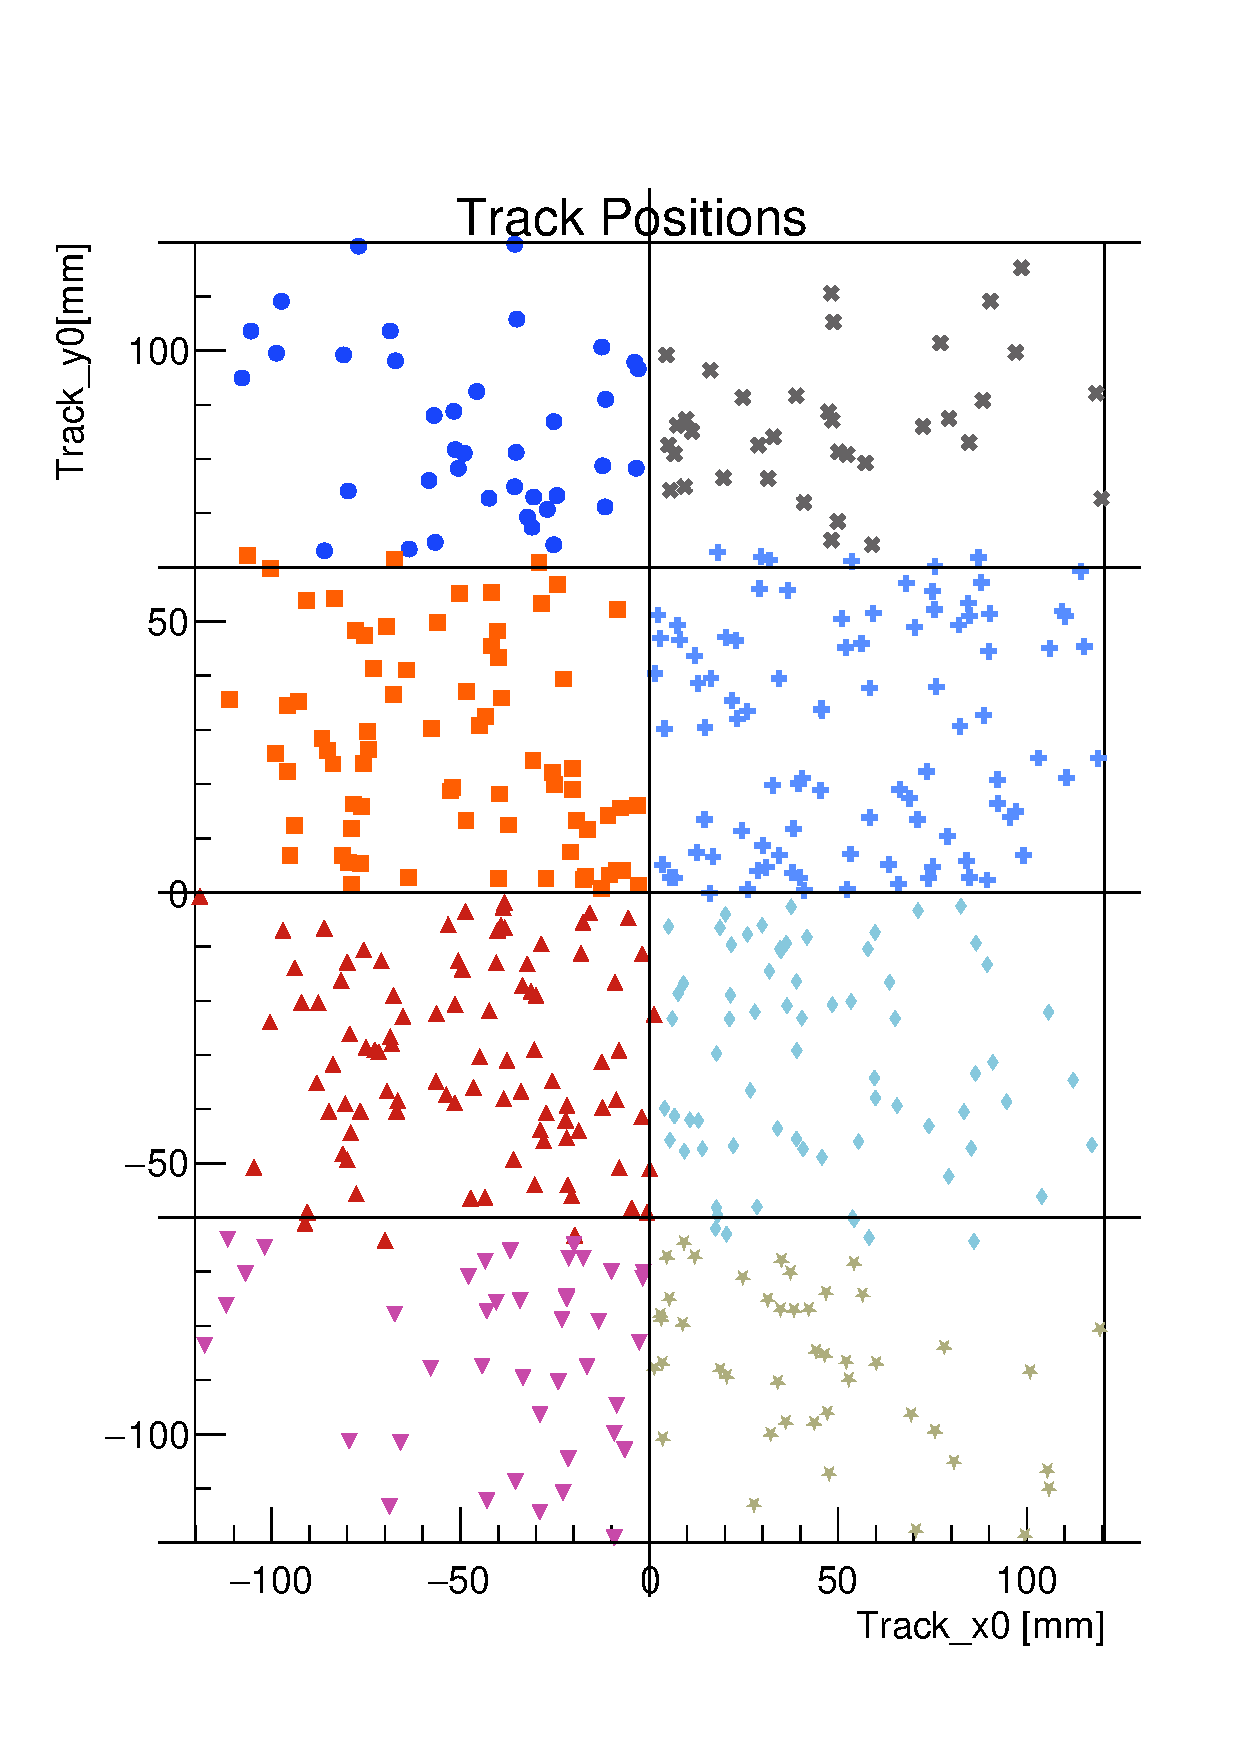
\includegraphics[height=0.8\textheight]{./ModuleLevelPlots/Positions_st0_truemodule0.pdf}
                \caption{500 Points at Station-1 colored according to modules}
            \end{figure}
        \end{column}
        \begin{column}{0.2\linewidth}
            \begin{figure}
                \hspace{-7cm}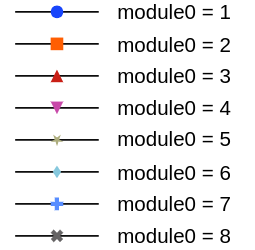
\includegraphics[scale=0.25]{./assets/image.png}
            \end{figure}
        \end{column}
    \end{columns}
\end{frame}

\begin{frame}{Where are the Module Boundaries?}
    \begin{figure}
        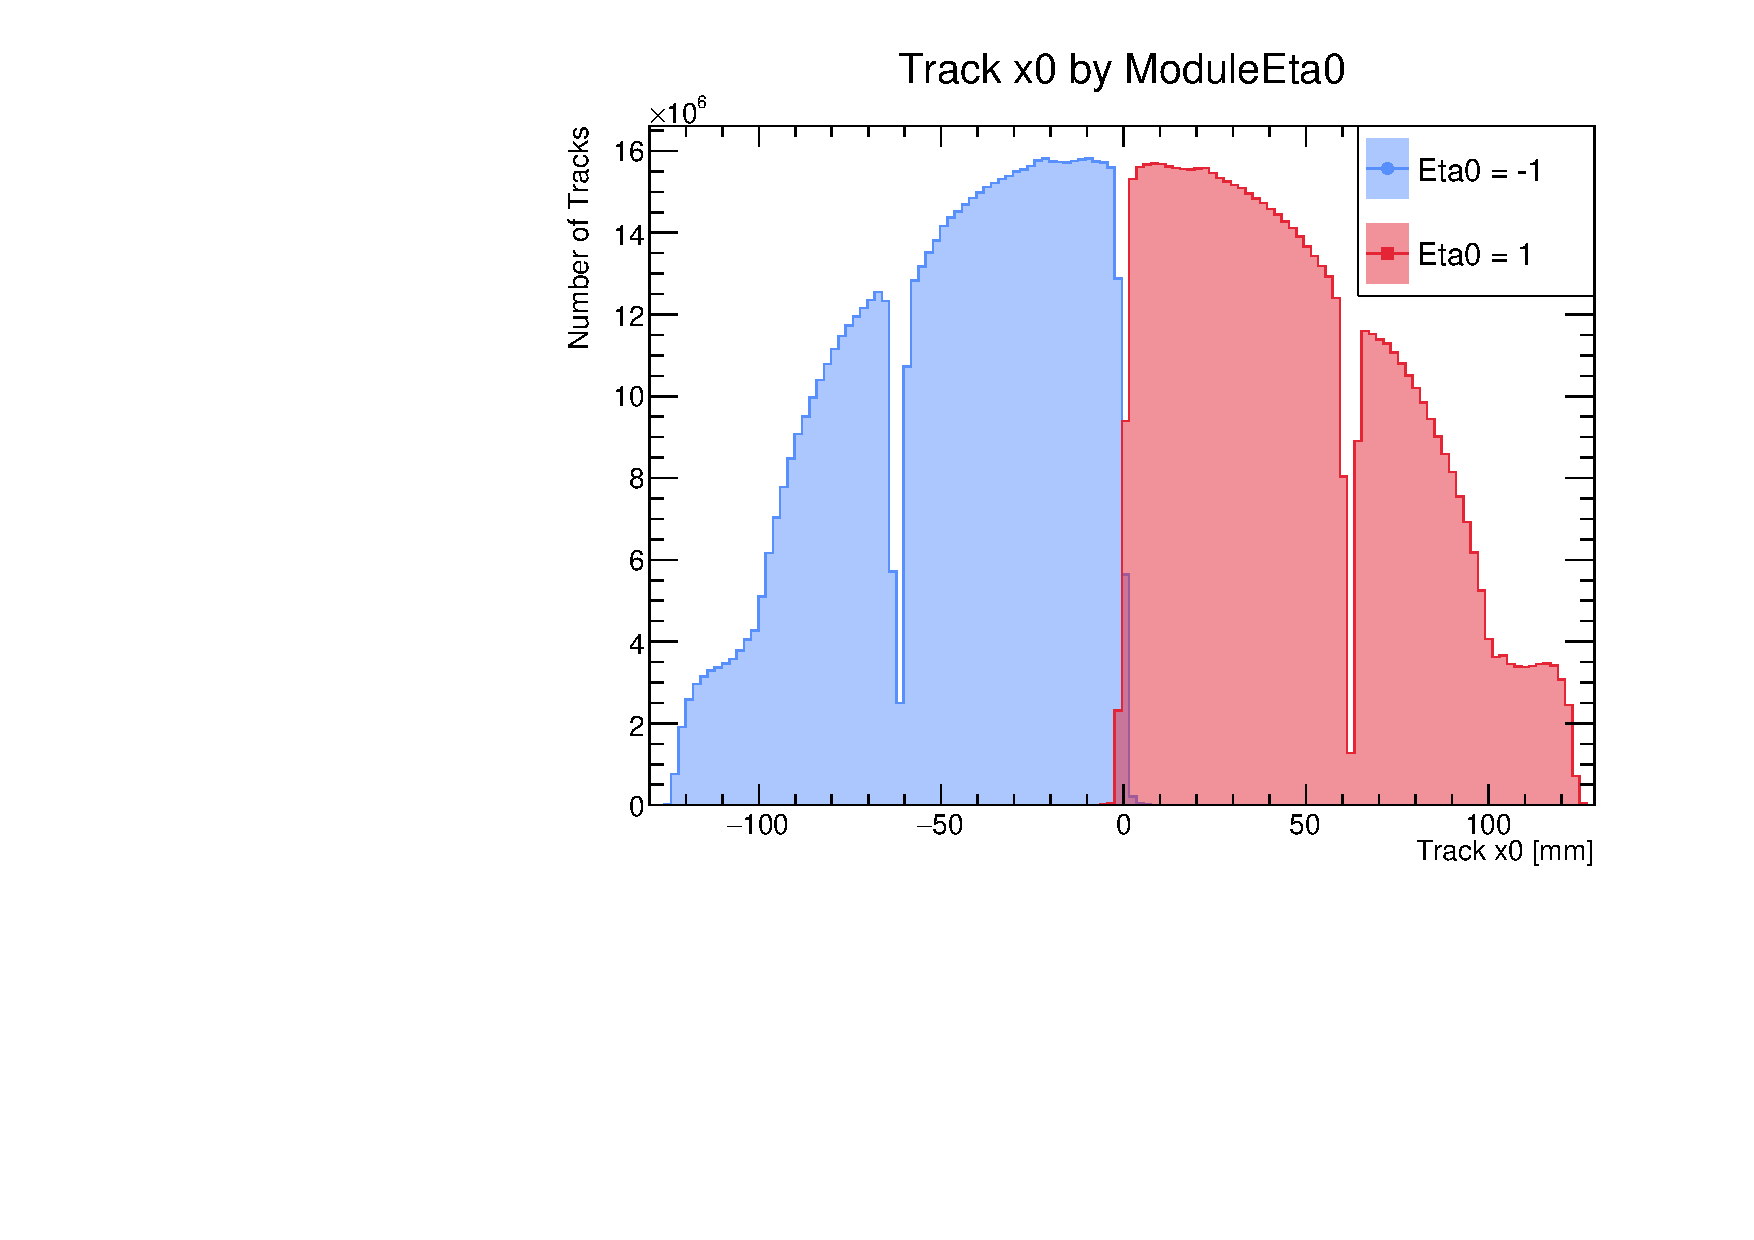
\includegraphics[width=\linewidth]{./ModuleLevelPlots/Track_x0_eta0.pdf}
        \caption{Track Positions at Station 1 colored by module\_eta0}
    \end{figure}
\end{frame}
\begin{frame}{Where are the Module Boundaries?}
    \begin{figure}
        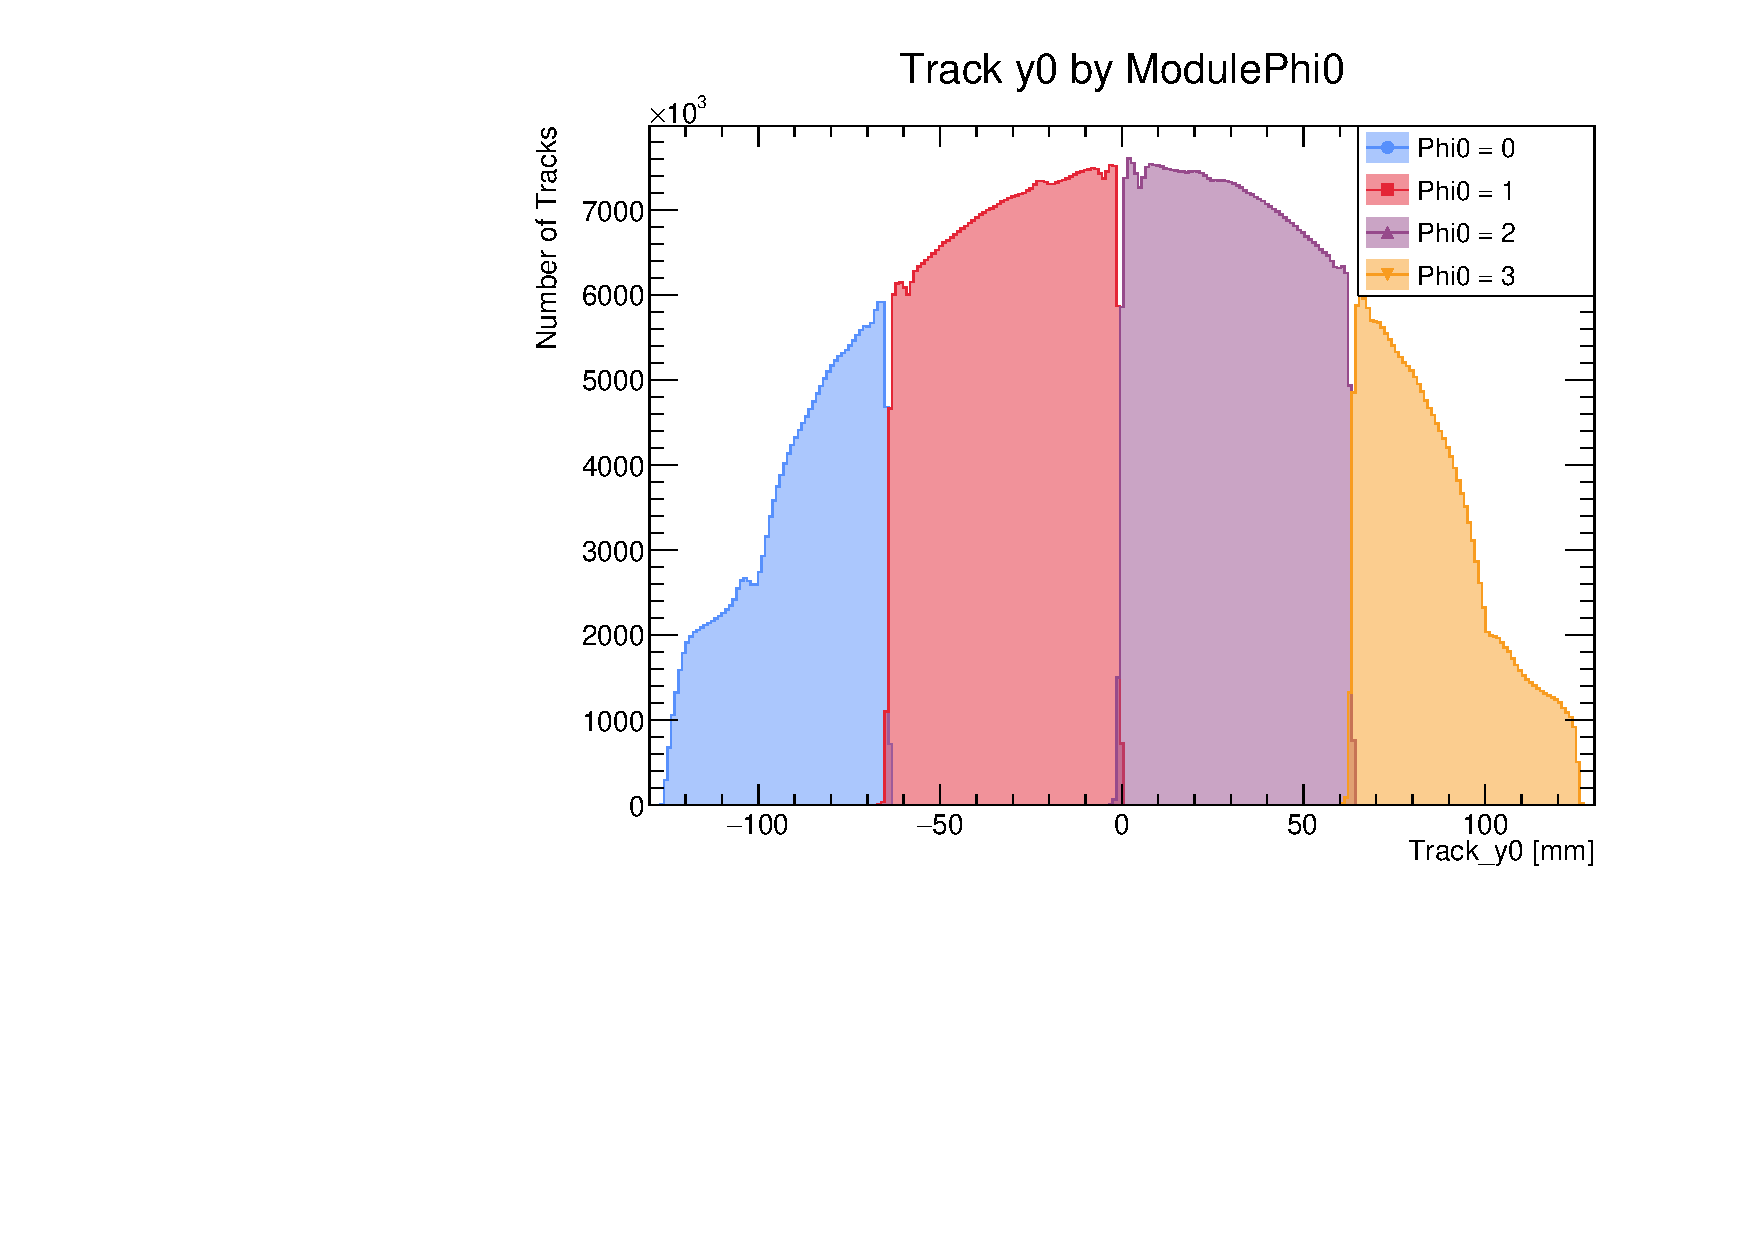
\includegraphics[width=\linewidth]{./ModuleLevelPlots/Track_y0_phi0.pdf}
        \caption{Track Positions at Station 1 colored by module\_phi0}
    \end{figure}
\end{frame}


\begin{frame}{Module Boundaries Schematic }
    \begin{figure}
        \hspace{-1cm}
        \begin{tikzpicture}[scale=0.24]
            % \draw[step=1cm,gray!30,very thin] (-12,-12) grid (12,12);

            \draw[-,thick] (0,-12) -- (0,12);
            \draw[-,thick] (-12,-12) -- (-12,12);
            \draw[-,thick] (12,-12) -- (12,12);


            \draw[-, thick] (-12, -12) -- (12, -12);
            \draw[-, thick] (-12, -6) -- (12, -6);
            \draw[-, thick] (-12, 0) -- (12, 0);
            \draw[-, thick] (-12, 6) -- (12, 6);
            \draw[-, thick] (-12, 12) -- (12, 12);

            \node[rectangle, draw=none, minimum size=1pt] at ( -6 , 9 )  {Module 1};
            \node[rectangle, draw=none, minimum size=1pt] at ( -6 , 3 )  {Module 2};
            \node[rectangle, draw=none, minimum size=1pt] at ( -6 , -3 ) {Module 3};
            \node[rectangle, draw=none, minimum size=1pt] at ( -6 , -9 ) {Module 4};

            \node[rectangle, draw=none, minimum size=1pt] at ( 6 , -9 )  {Module 5};
            \node[rectangle, draw=none, minimum size=1pt] at ( 6 , -3 )  {Module 6};
            \node[rectangle, draw=none, minimum size=1pt] at ( 6 , 3 )   {Module 7};
            \node[rectangle, draw=none, minimum size=1pt] at ( 6 , 9 )   {Module 8};

            \draw[->, thick] (-13, -13) -- (-13, 13.5) node[above right] {$y$};
            \draw[->, thick] (-13, -13) -- (13, -13) node[right] {$x$};
            
            \draw[- , thick] (-13, -12) -- (-12.5, -12) node[left=0.1cm] {-120}; 
            \draw[- , thick] (-13,  -6) -- (-12.5,  -6) node[left=0.1cm] {-60}; 
            \draw[- , thick] (-13,   0) -- (-12.5,   0) node[left=0.1cm] {0}; 
            \draw[- , thick] (-13,   6) -- (-12.5,   6) node[left=0.1cm] {60}; 
            \draw[- , thick] (-13,  12) -- (-12.5,  12) node[left=0.1cm] {120}; 

            \draw[- , thick] (-12, -13) -- (-12, -12.5) node[below=0.1cm] {-120};
            \draw[- , thick] (0,   -13) -- (0,   -12.5) node[below=0.1cm] {0}; 
            \draw[- , thick] (12,  -13) -- (12,  -12.5) node[below=0.1cm] {12}; 

            \node at (-17, -9) {Phi = 0};
            \node at (-17, -3) {Phi = 1};
            \node at (-17, +3) {Phi = 2};
            \node at (-17, +9) {Phi = 3};

            \node at (-6, -14.7) {Eta = -1};
            \node at (+6, -14.7) {Eta = +1};

            % \node[rectangle, draw=none, minimum size=1pt] at ( -6 , 9 )  {Module 1};
        \end{tikzpicture}
        \caption{Module Boundaries Schematic. Numbering borrowed from Angela's Schematic}
    \end{figure}
\end{frame}

\begin{frame}{Accuracy of Module Splits}
    \begin{itemize}
        \item Since 2023 does not have the module\_eta0 / phi0 entries we approximate them using the above schematic.
    \end{itemize}
    \begin{figure}
        \centering
        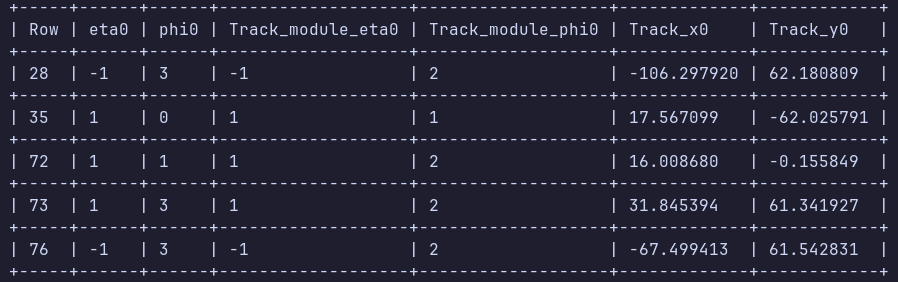
\includegraphics[width=1.0\linewidth]{./assets/ModuleMismatch.png}
        \caption{Module Calculation mismatch in run 016635}
    \end{figure}   
    \begin{itemize}
        \item Mismatch are within $\pm$ 5 mm of the borders
        \item Number of Mismatches:  587982  out of  13601766 i.e 4.3\%
    \end{itemize}
\end{frame}

\begin{frame}{Revisiting Positions at Station 1}
    \begin{columns}
        \begin{column}{1.2\linewidth}
            \begin{figure}
                \centering
                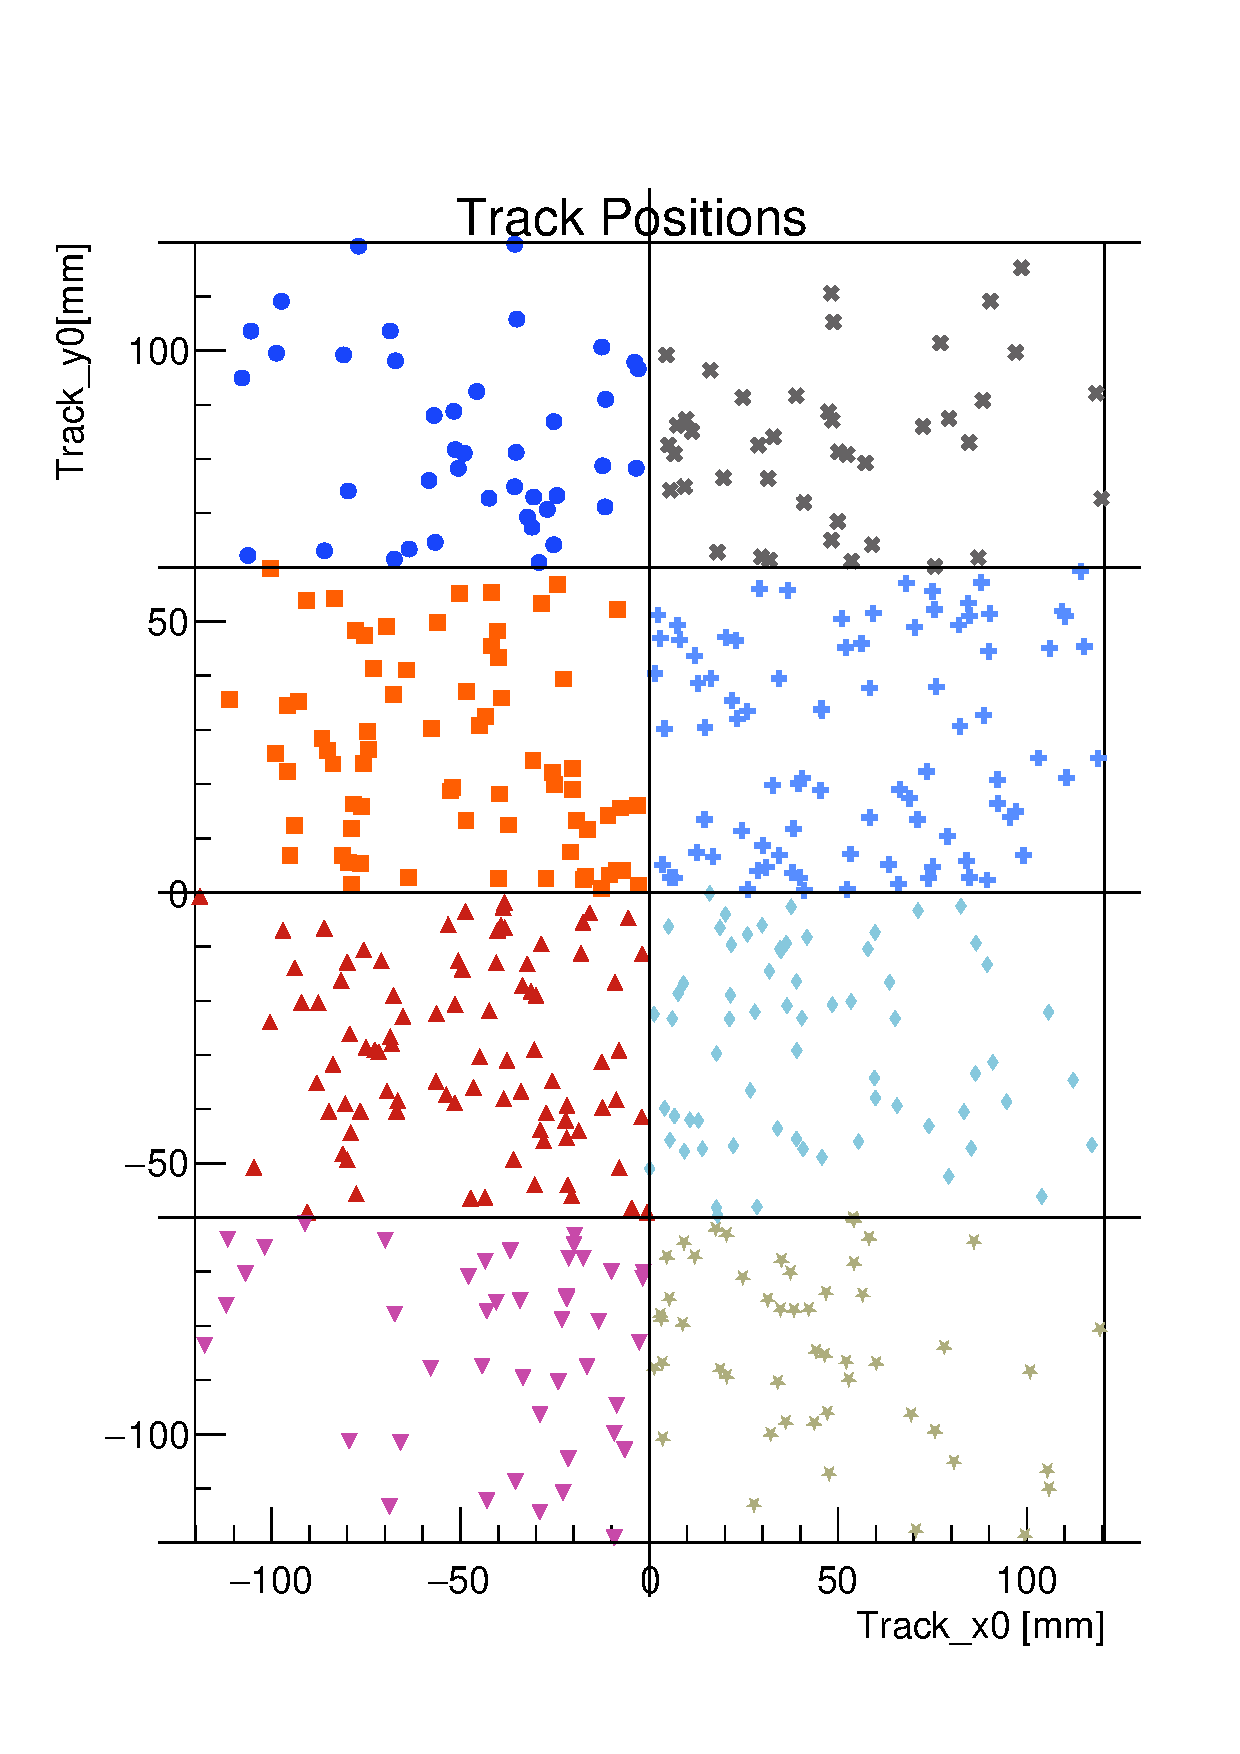
\includegraphics[height=0.8\textheight]{./ModuleLevelPlots/Positions_st0_module0.pdf}
                \caption{500 Points at Station 1 colored by Module number at Station 1}
            \end{figure}
        \end{column}
        \begin{column}{0.2\linewidth}
            \begin{figure}
                \hspace{-7cm}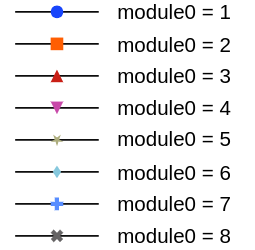
\includegraphics[scale=0.25]{./assets/image.png}
            \end{figure}
        \end{column}
    \end{columns}
\end{frame}

\begin{frame}{Where do they end up in Station 2?}
    \begin{columns}
        \begin{column}{1.2\linewidth}
            \begin{figure}
                \centering
                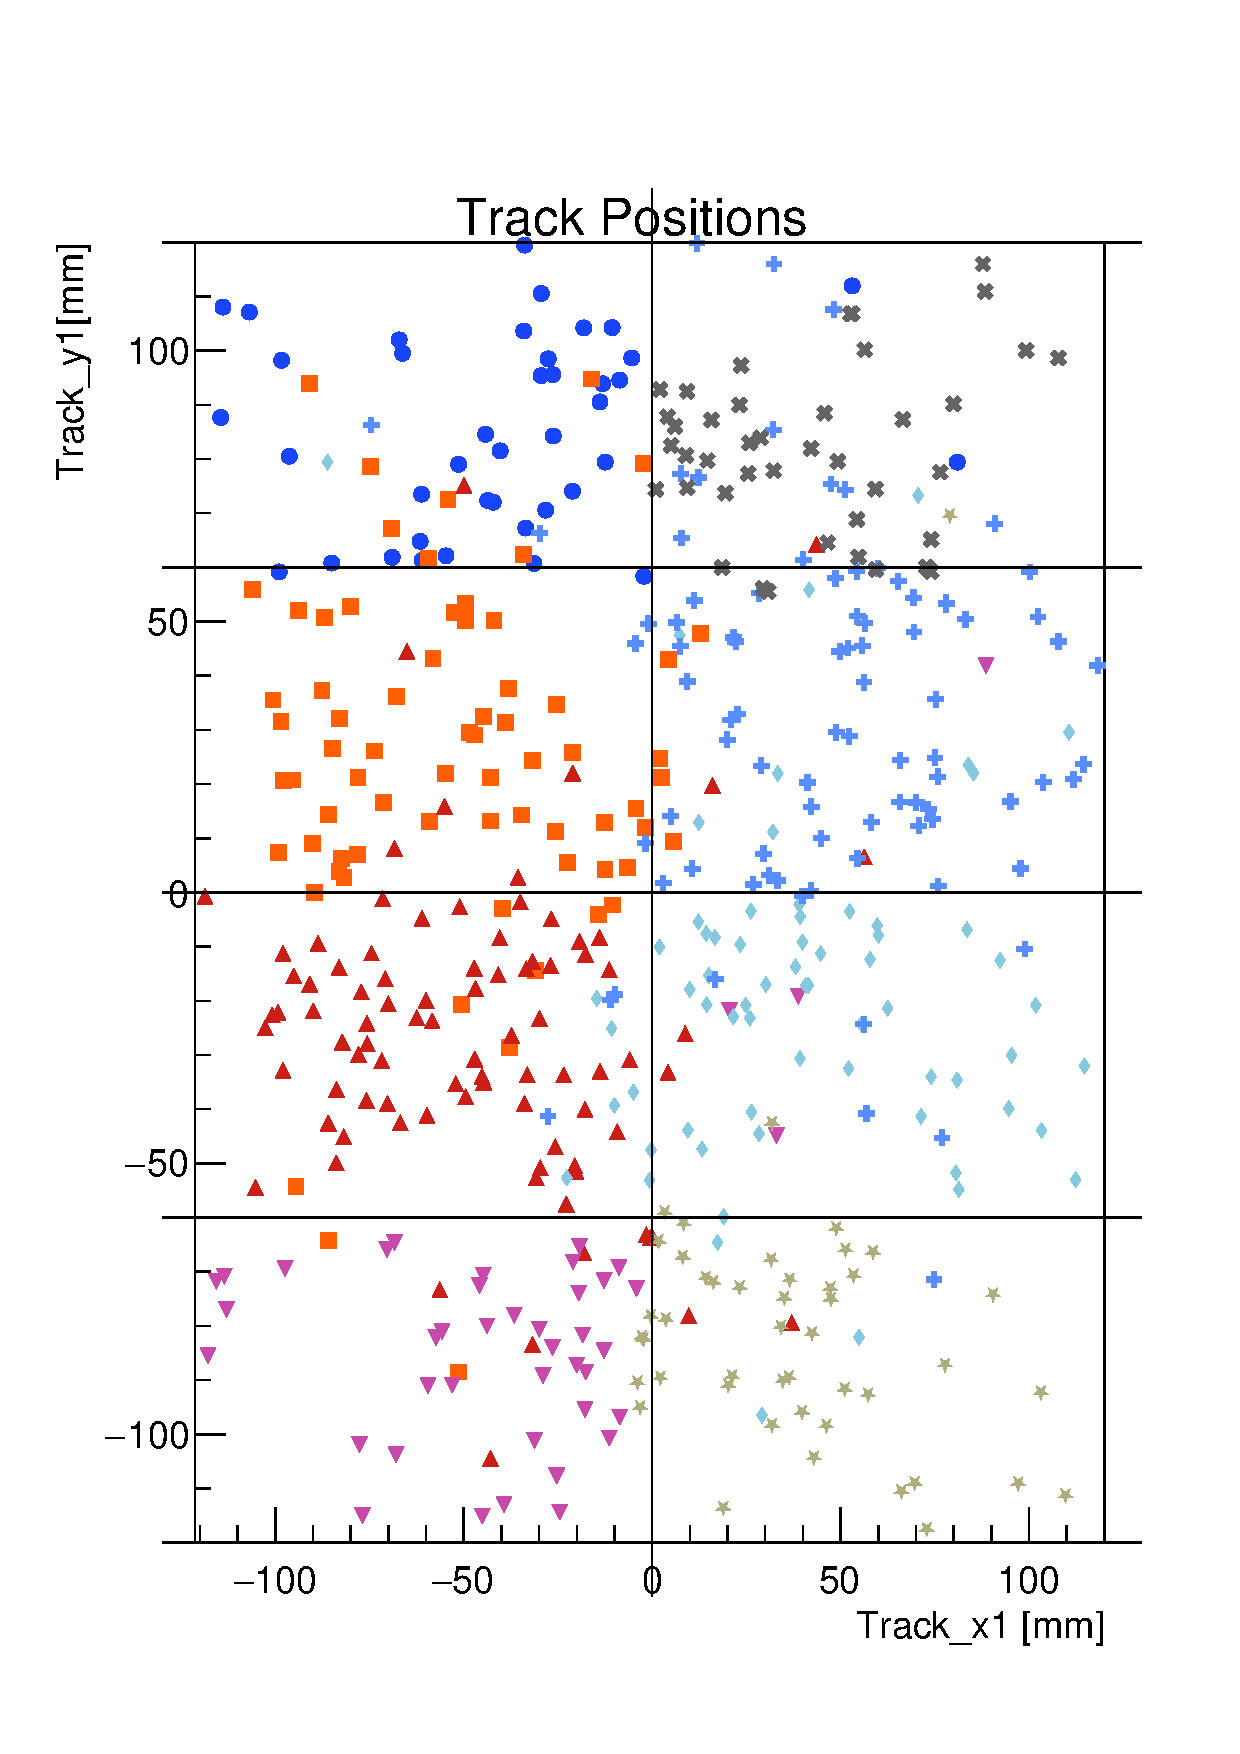
\includegraphics[height=0.8\textheight]{./ModuleLevelPlots/Positions_st1_module0.pdf}
                \caption{500 Points at Station 3 colored by Module number at Station 1}
            \end{figure}
        \end{column}
        \begin{column}{0.2\linewidth}
            \begin{figure}
                \hspace{-7cm}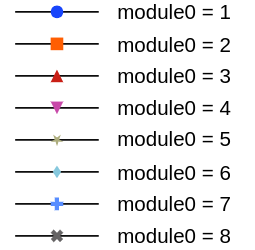
\includegraphics[scale=0.25]{./assets/image.png}
            \end{figure}
        \end{column}
    \end{columns}
\end{frame}

\begin{frame}{Transfer Heatmap in 2023}
    \begin{columns}
        \begin{column}{0.85\linewidth}
            \begin{figure}
                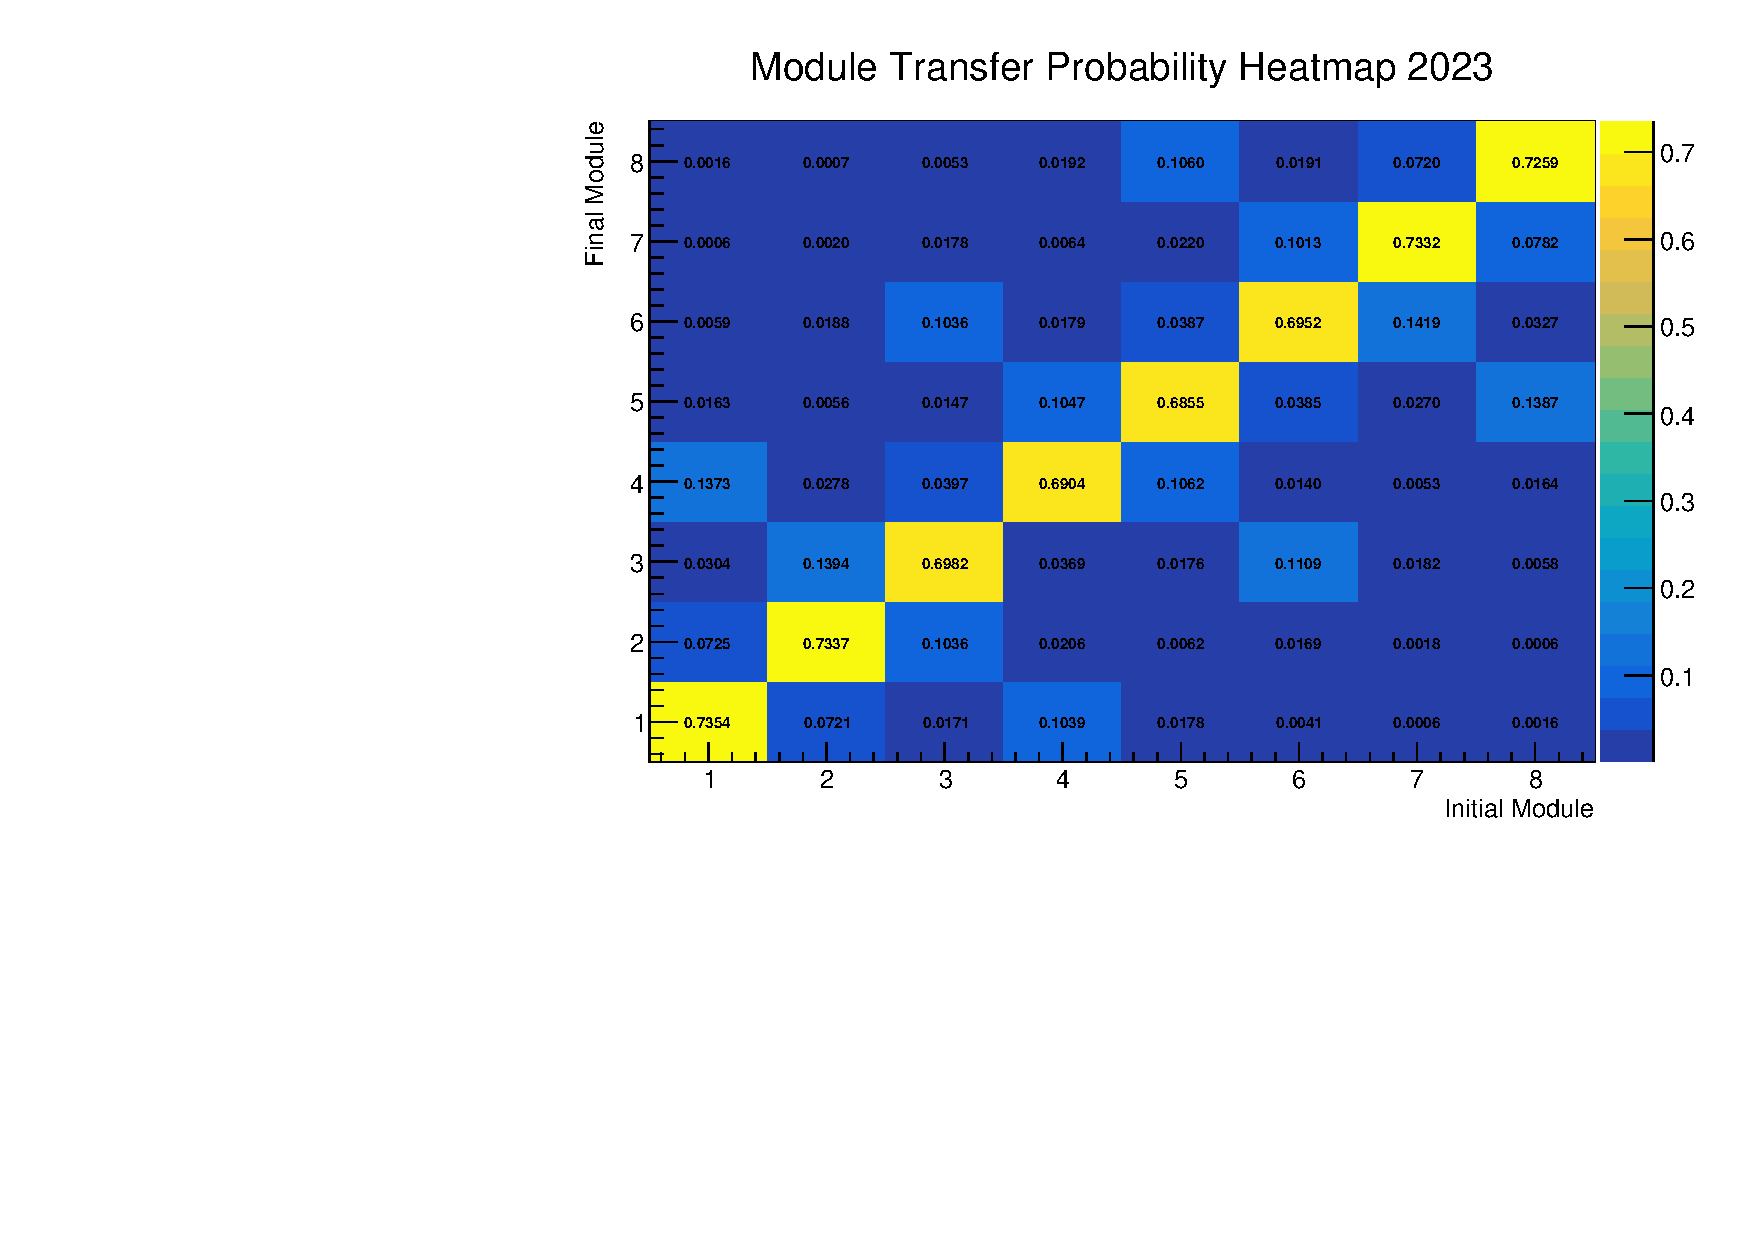
\includegraphics[width=0.9\linewidth]{./ModuleLevelPlots/st0_module_number vs st1_module_number_prob_2023.pdf}
                \caption{Probability of Transfer from Initial Module (at Station 1) to Final Module (at Station 2) based on 2023 Data}
            \end{figure}
        \end{column}
        \begin{column}{0.2\linewidth}
            \begin{figure}
                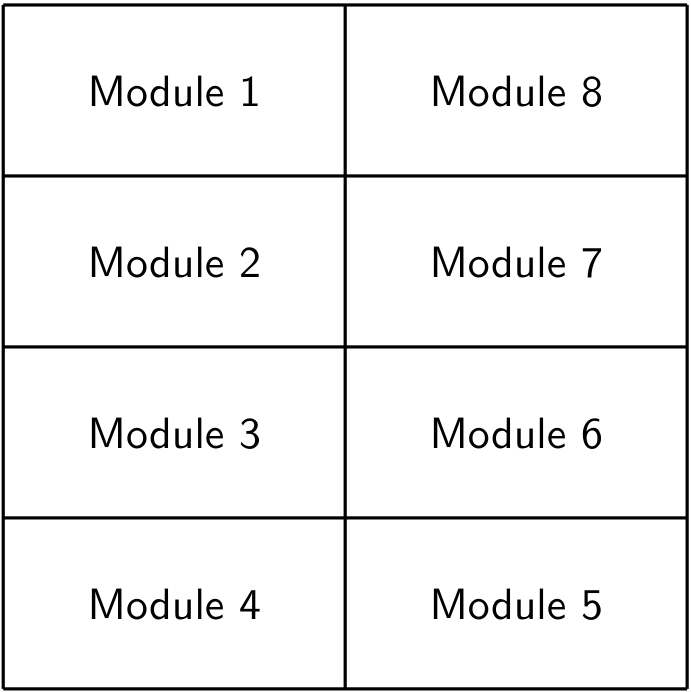
\includegraphics[width=\linewidth]{./assets/ModuleThumbnail.png}
            \end{figure}
        \end{column}
    \end{columns}
    \begin{itemize}
        \small
        \item Most probable transfer is to the same module followed by adjacent.
        \item Module 2,3,6,7 (central) are more likey to transfer to another central module. [Phrase this better]
    \end{itemize}
\end{frame}

\begin{frame}{Transfer Heatmap in 2024}
    \begin{figure}
        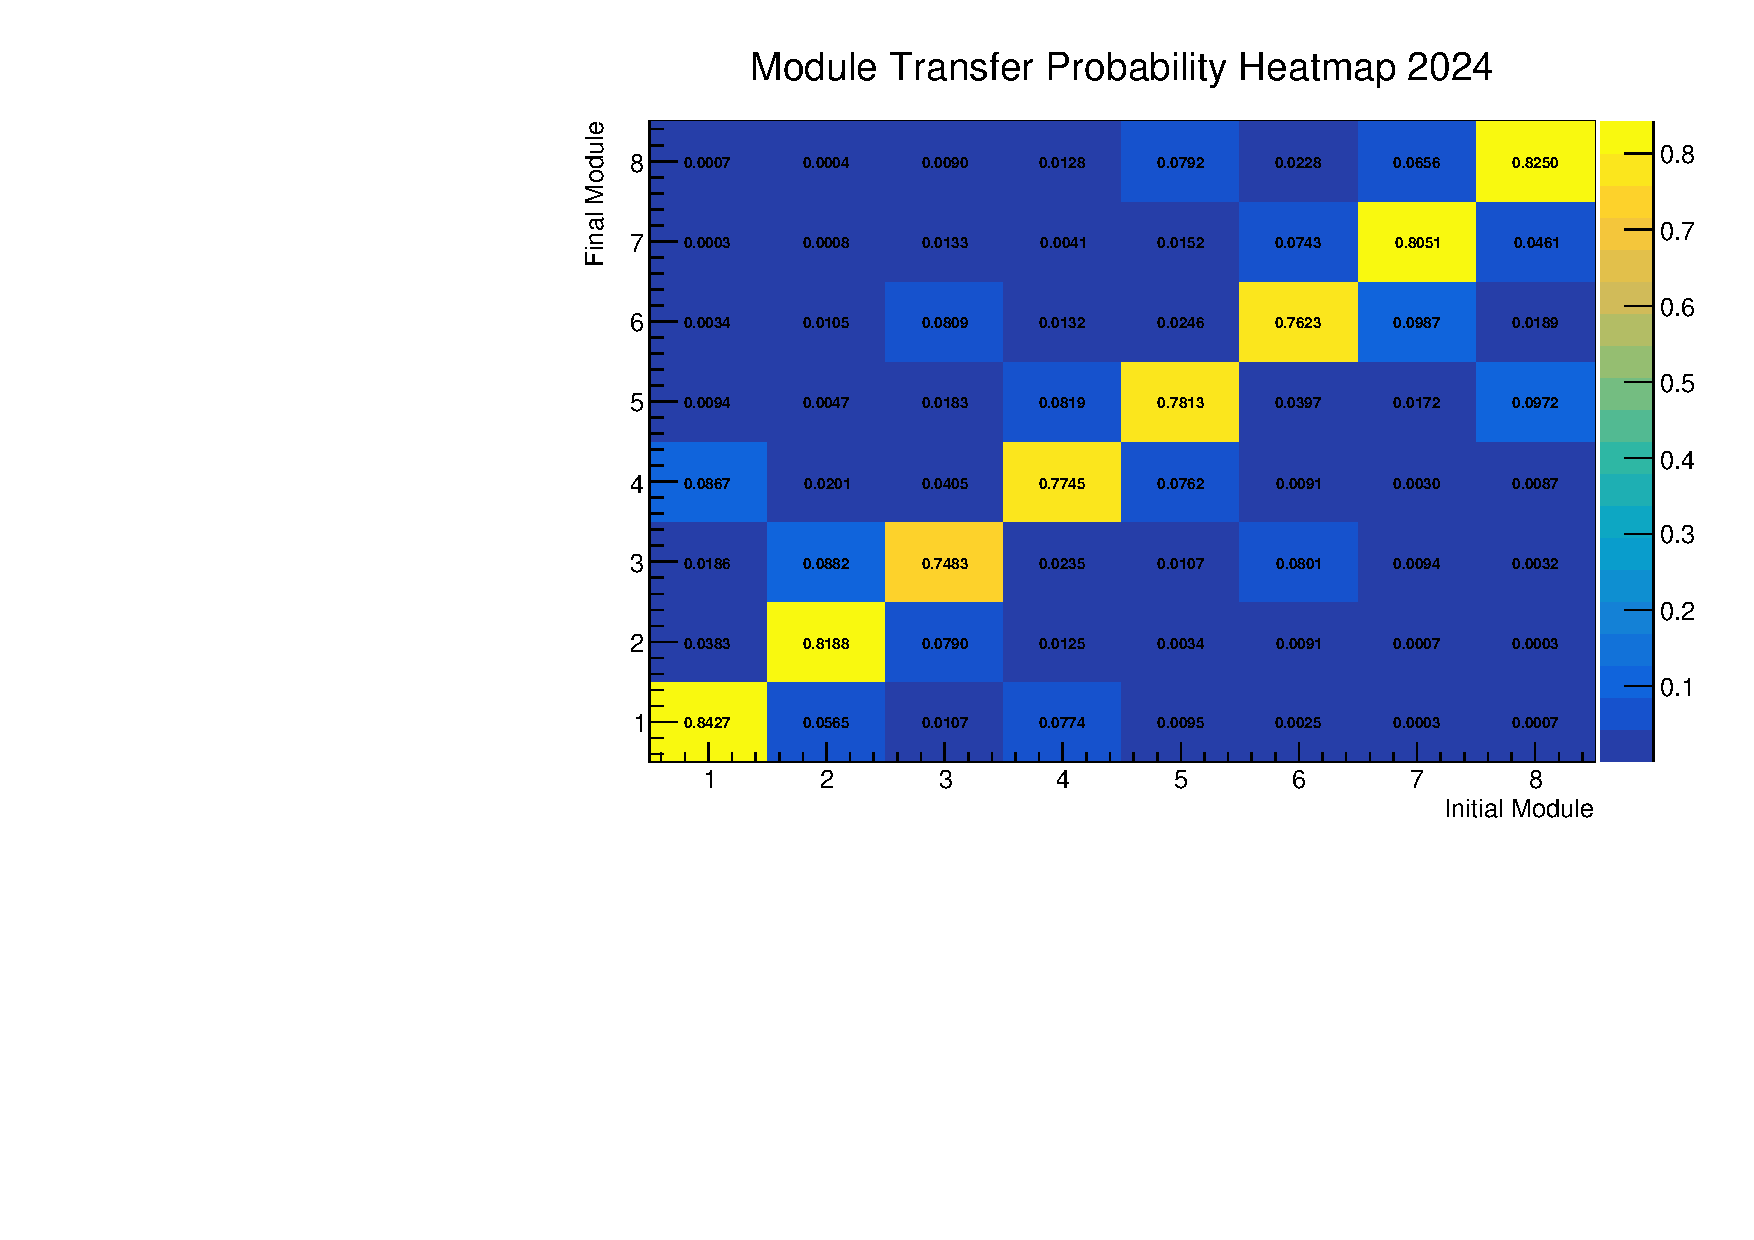
\includegraphics[width=0.8\linewidth]{./ModuleLevelPlots/st0_module_number vs st1_module_number_prob_2024.pdf}
        \caption{Probability of Transfer from Initial Module (at Station 1) to Final Module (at Station 2) based on 2024 data}
    \end{figure}
    \begin{itemize}
        \small
        \item Much higher Probability of Transfer to the same module
        \item In general less module transfers in 2024.
    \end{itemize}
\end{frame}

\begin{frame}{Transfer Heatmap Ratio }
    \begin{figure}
        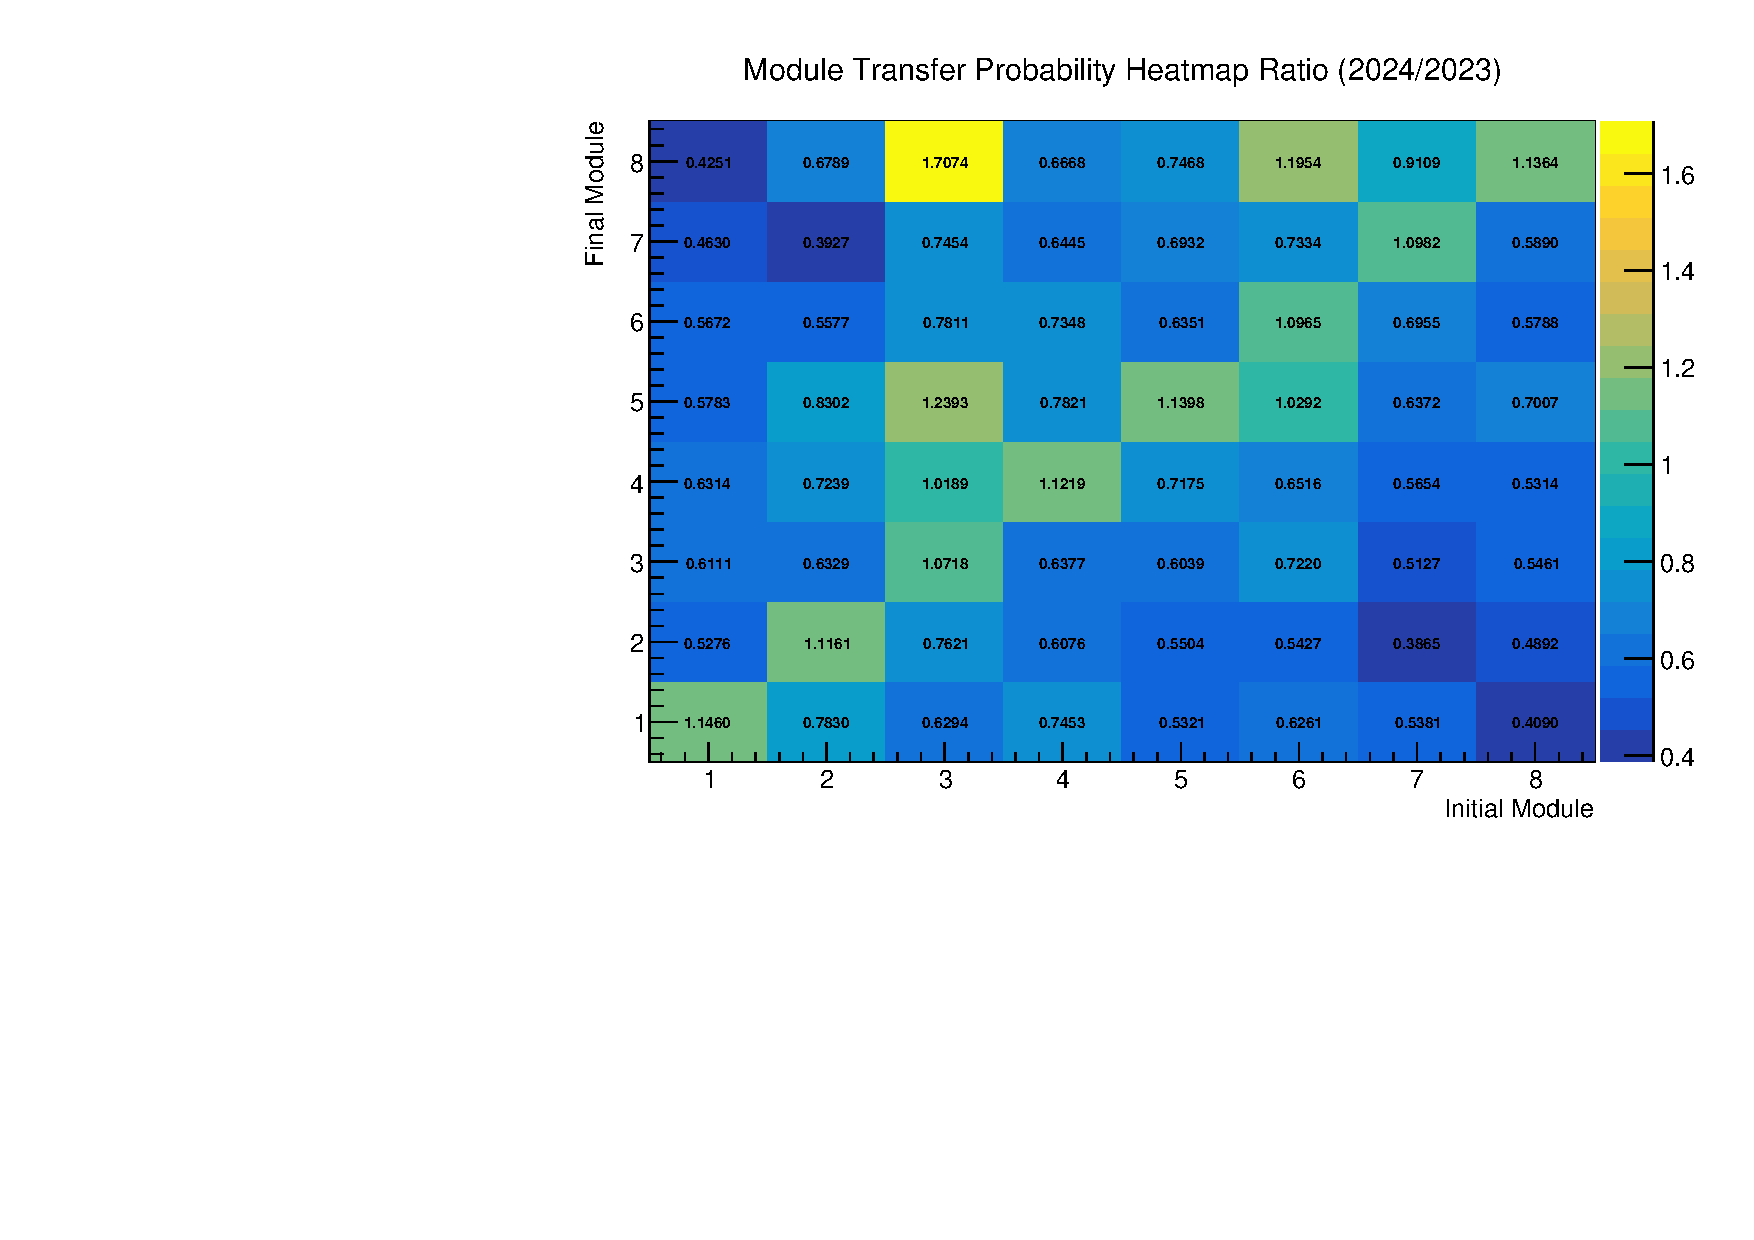
\includegraphics[width=0.86\linewidth]{./ModuleLevelPlots/st0_module_number vs st1_module_number_prob_ratio.pdf}
        \caption{Ratio of Probability of Transfer from Initial Module (at Station 1) to Final Module (at Station 2) }
    \end{figure}
    \begin{itemize}
        \small
        \item 2024 has a higher probability of transfer to the same module
        \item Module 3 and 6 seem to be transferring into 8 more [Why?]
    \end{itemize}

\end{frame}


\begin{frame}{Transfer Histograms}
    \begin{figure}
        \centering
        \begin{subfigure}[t]{0.49\linewidth}
            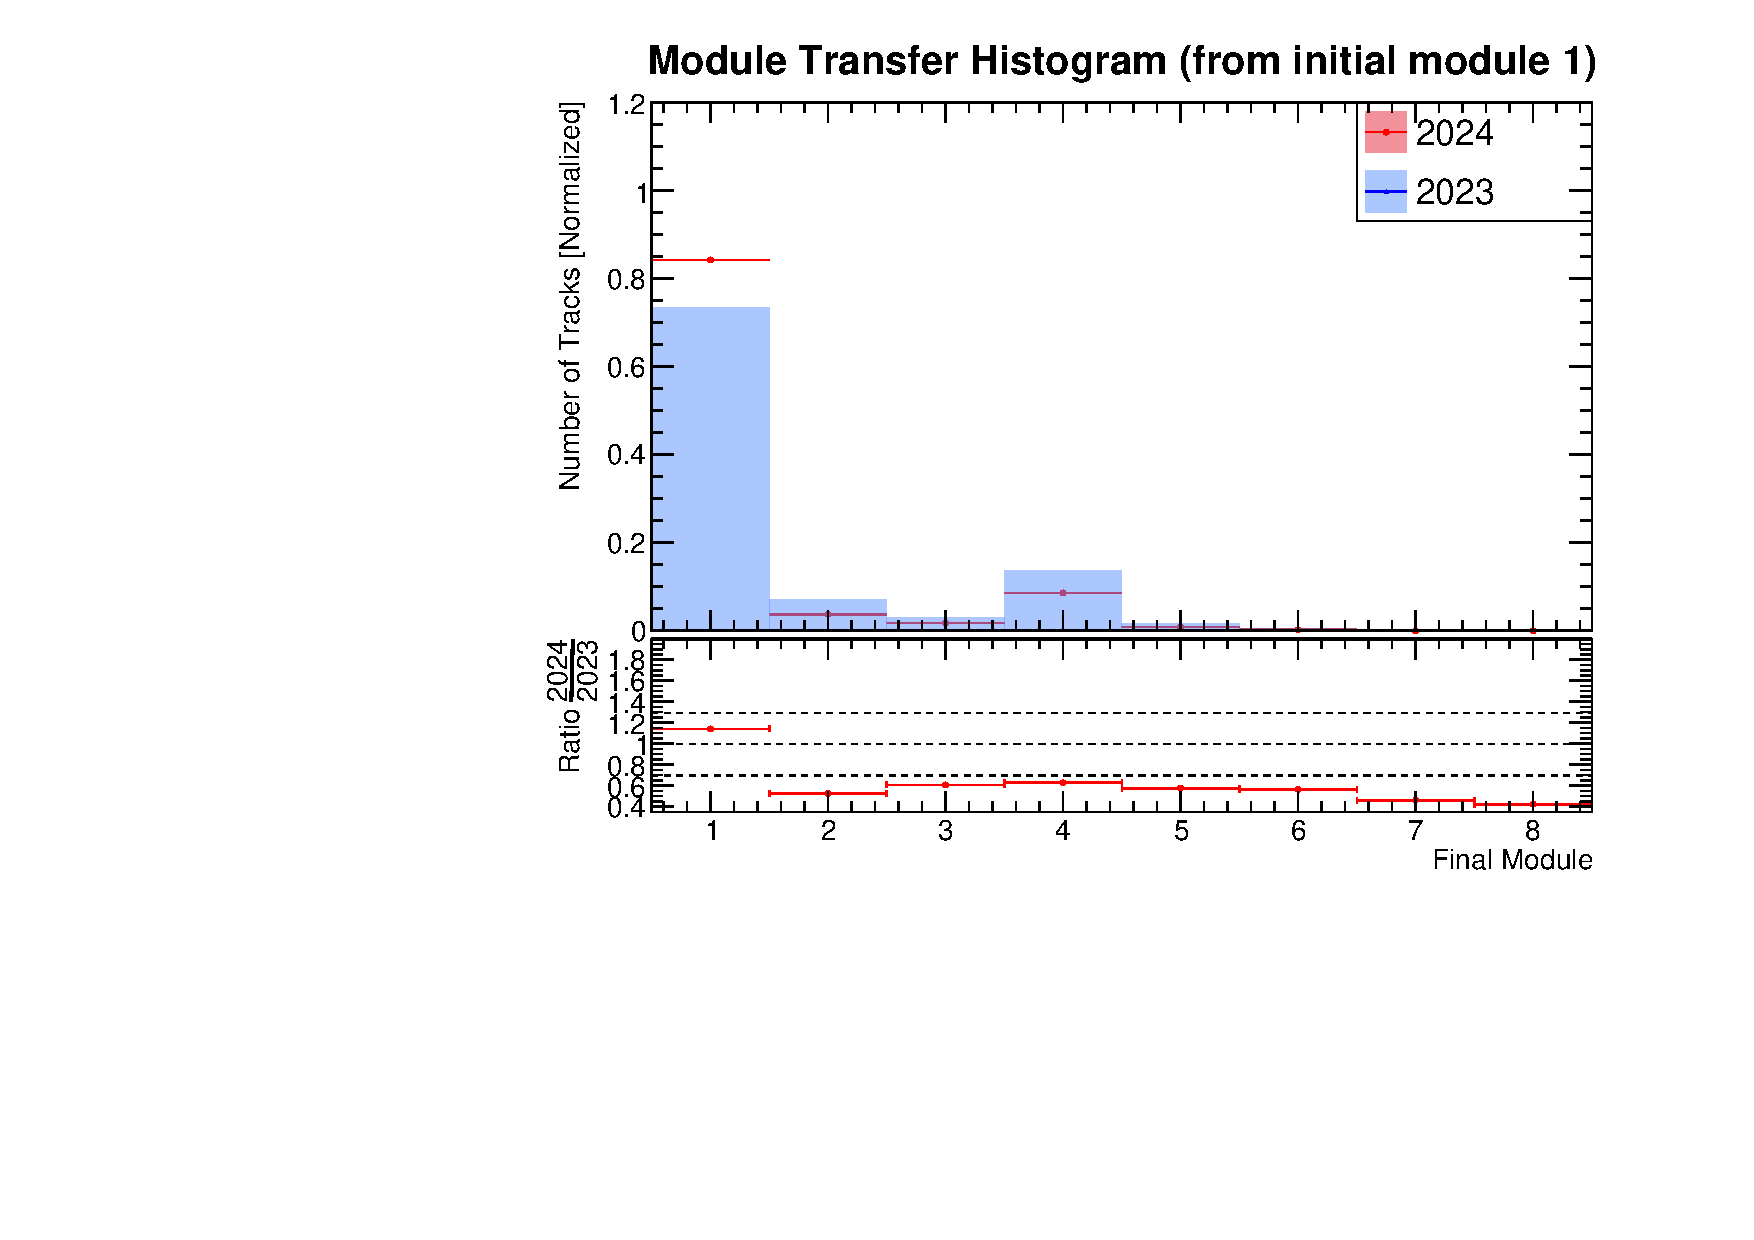
\includegraphics[width=\linewidth]{./ModuleLevelPlots/final_module_from_st0_module1.pdf}
        \end{subfigure}
        \begin{subfigure}[t]{0.49\linewidth}
            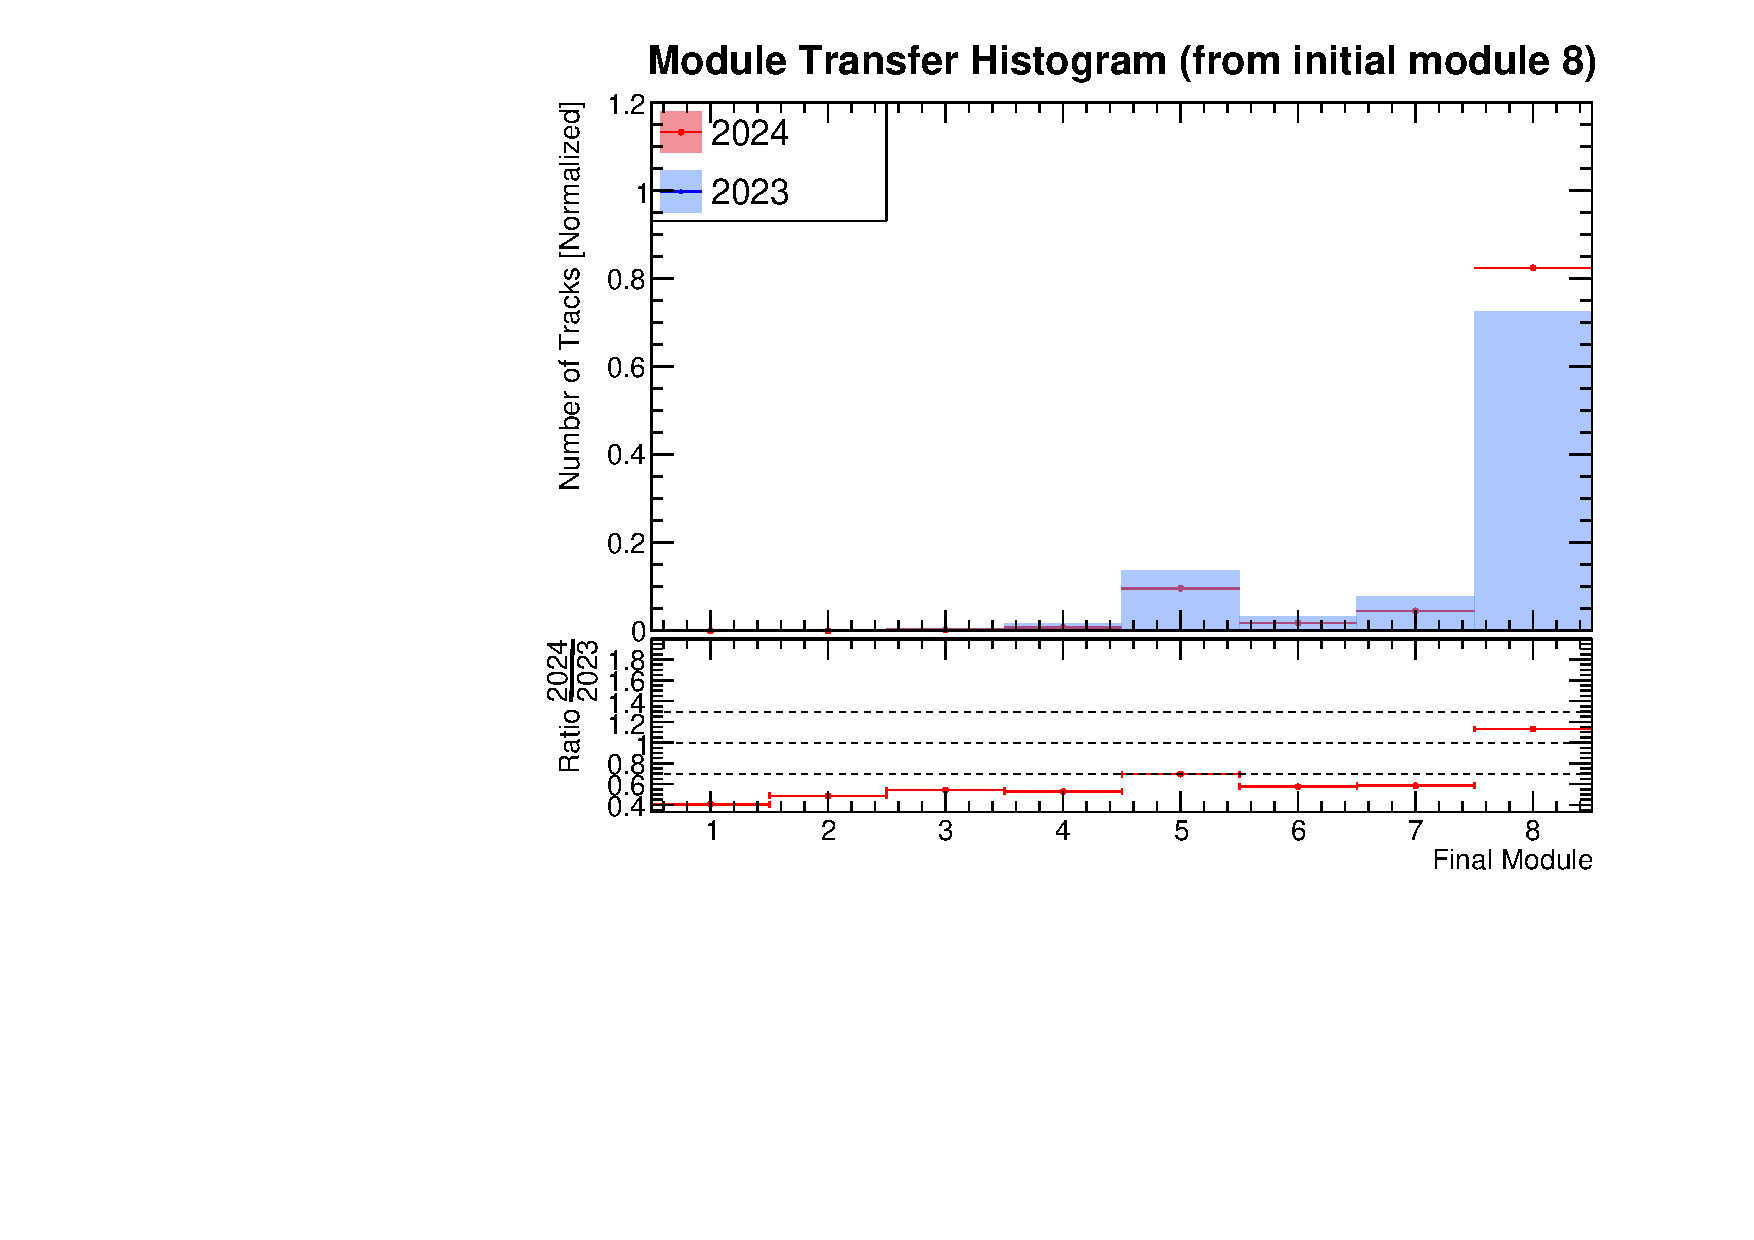
\includegraphics[width=\linewidth]{./ModuleLevelPlots/final_module_from_st0_module8.pdf}
        \end{subfigure}

        \begin{subfigure}[t]{0.49\linewidth}
            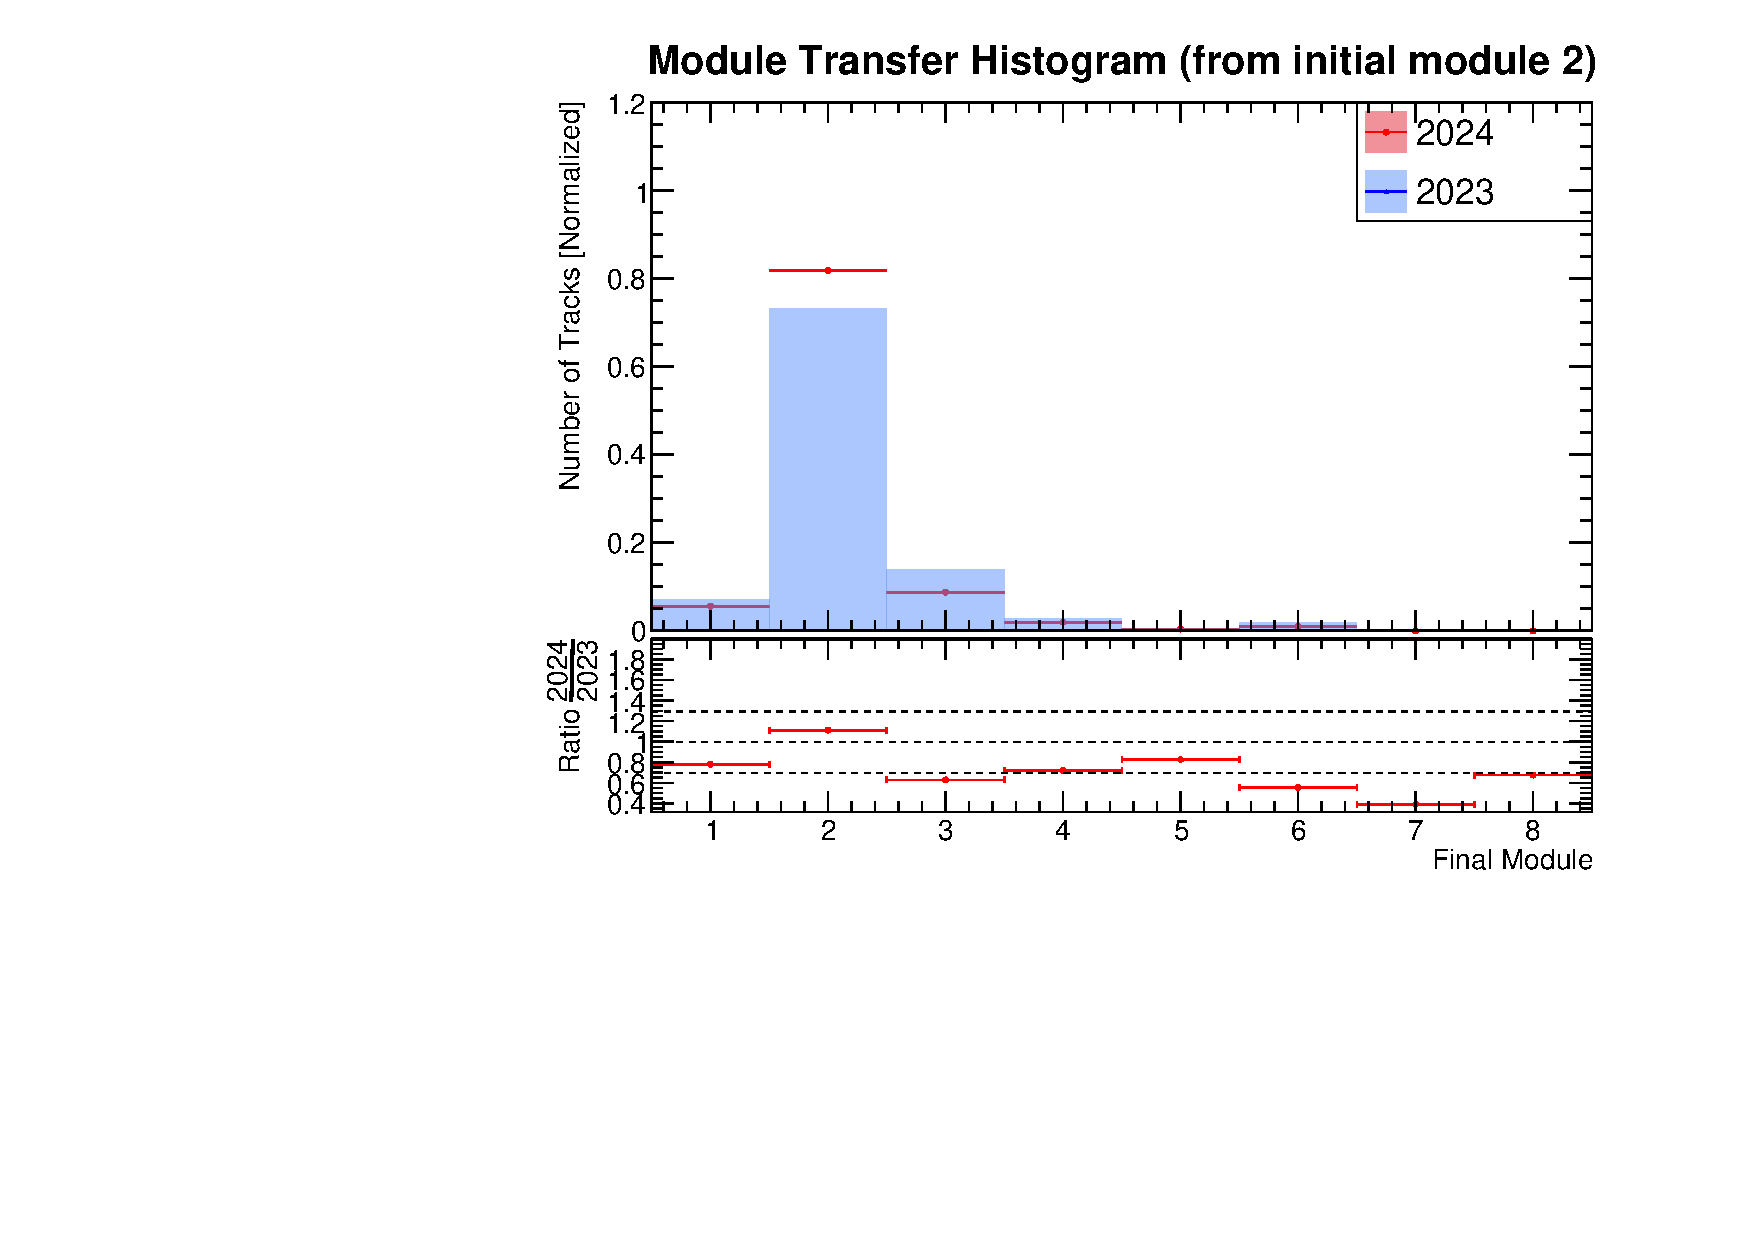
\includegraphics[width=\linewidth]{./ModuleLevelPlots/final_module_from_st0_module2.pdf}
        \end{subfigure}
        \begin{subfigure}[t]{0.49\linewidth}
            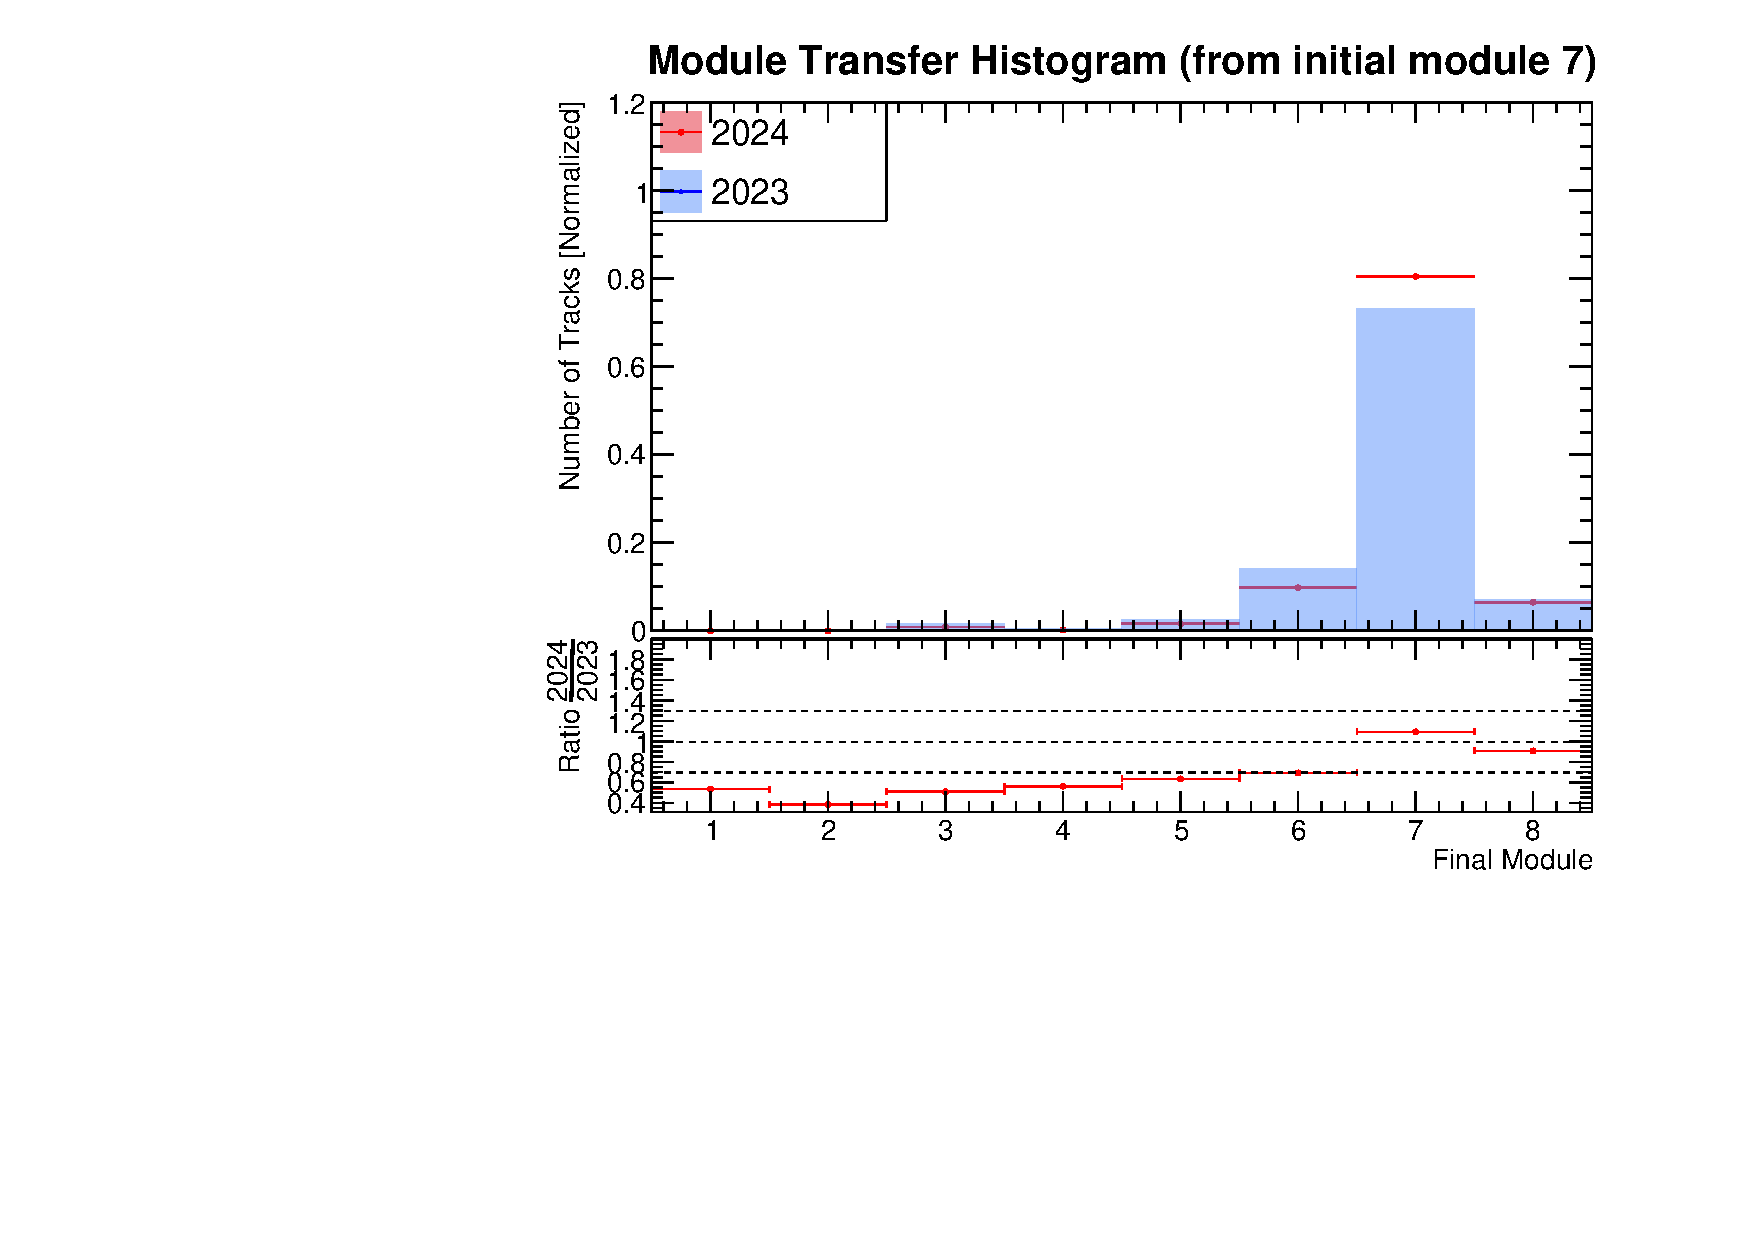
\includegraphics[width=\linewidth]{./ModuleLevelPlots/final_module_from_st0_module7.pdf}
        \end{subfigure}
    \end{figure}
    \vspace{-0.5cm}
    \scriptsize Note: 1-4 transfer seem significant? and 8-5 transfer seem significant?
\end{frame}

\begin{frame}{Transfer Histograms [Contd.]}
    \begin{figure}
        \centering
        \begin{subfigure}[t]{0.49\linewidth}
            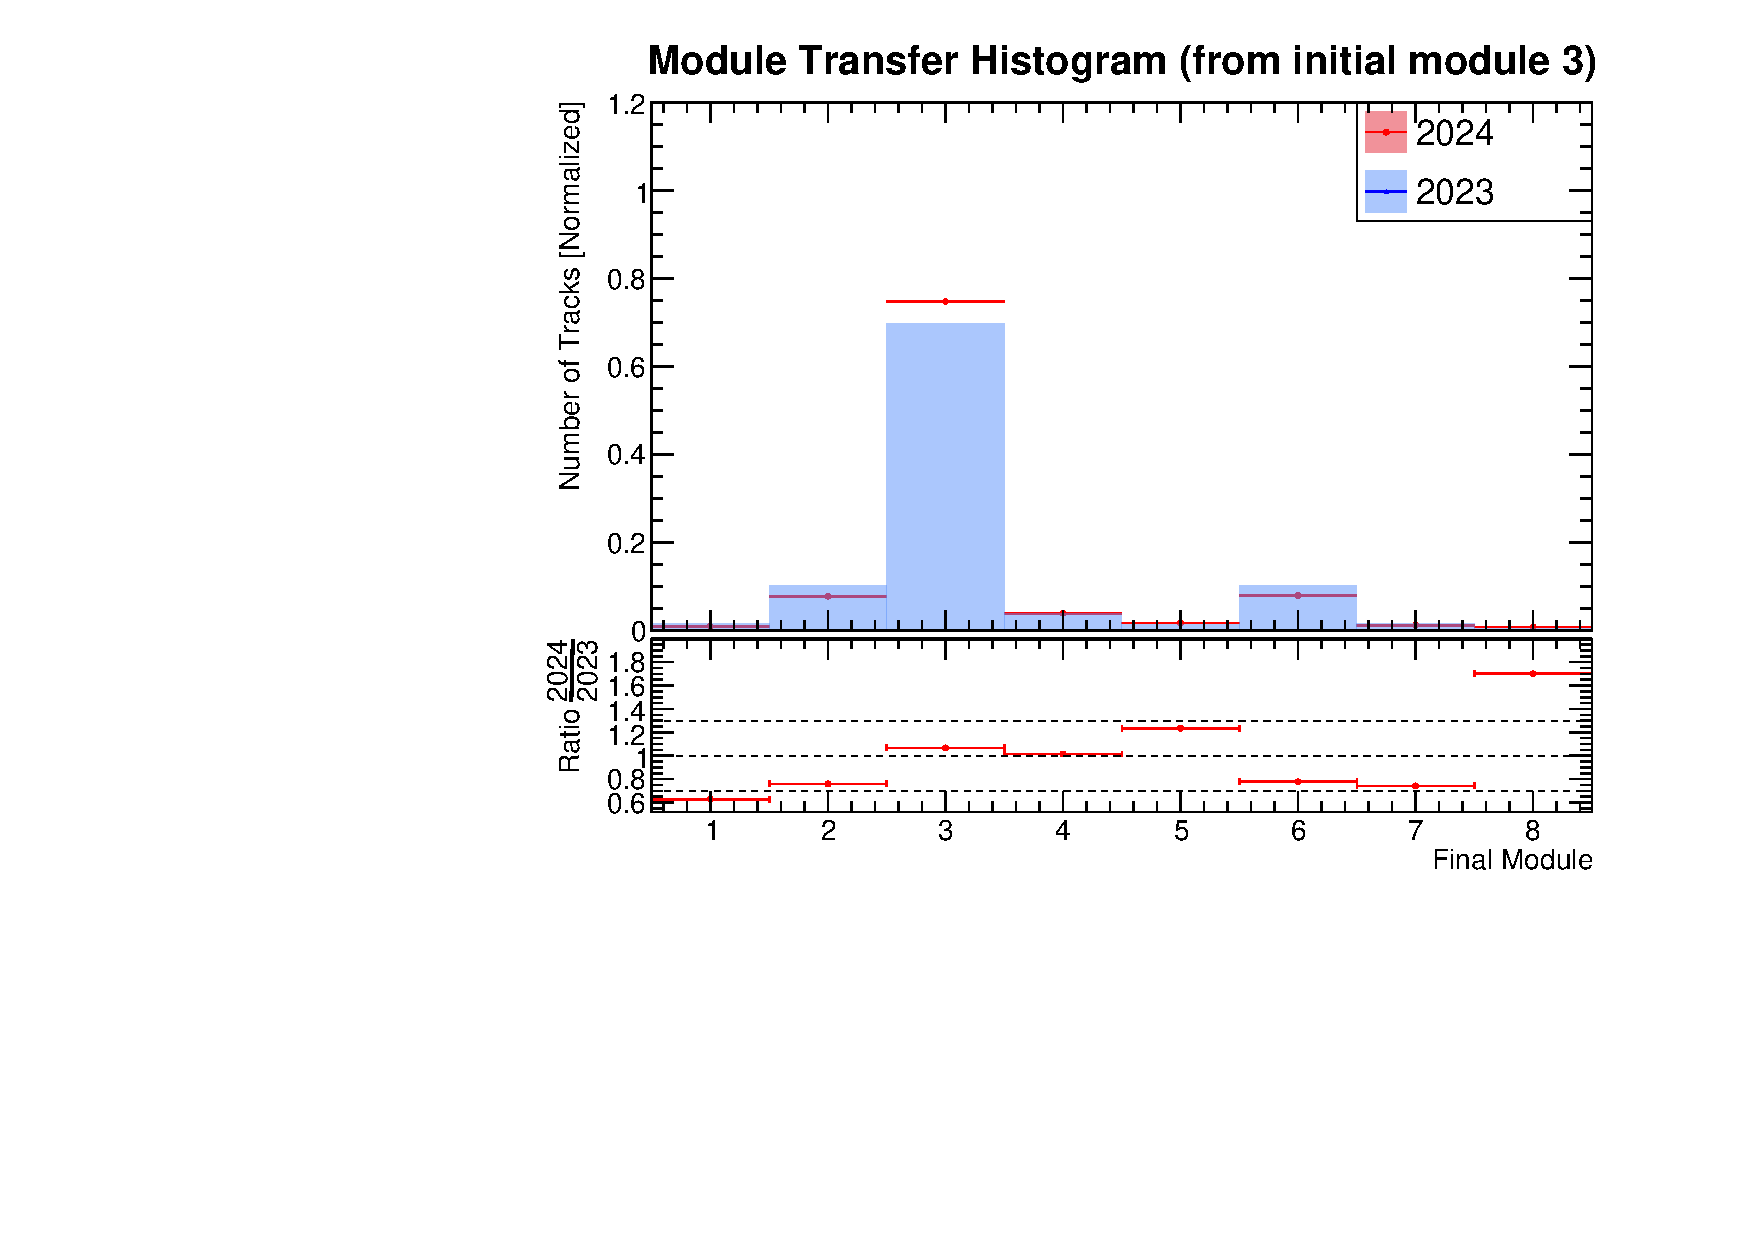
\includegraphics[width=\linewidth]{./ModuleLevelPlots/final_module_from_st0_module3.pdf}
        \end{subfigure}
        \begin{subfigure}[t]{0.49\linewidth}
            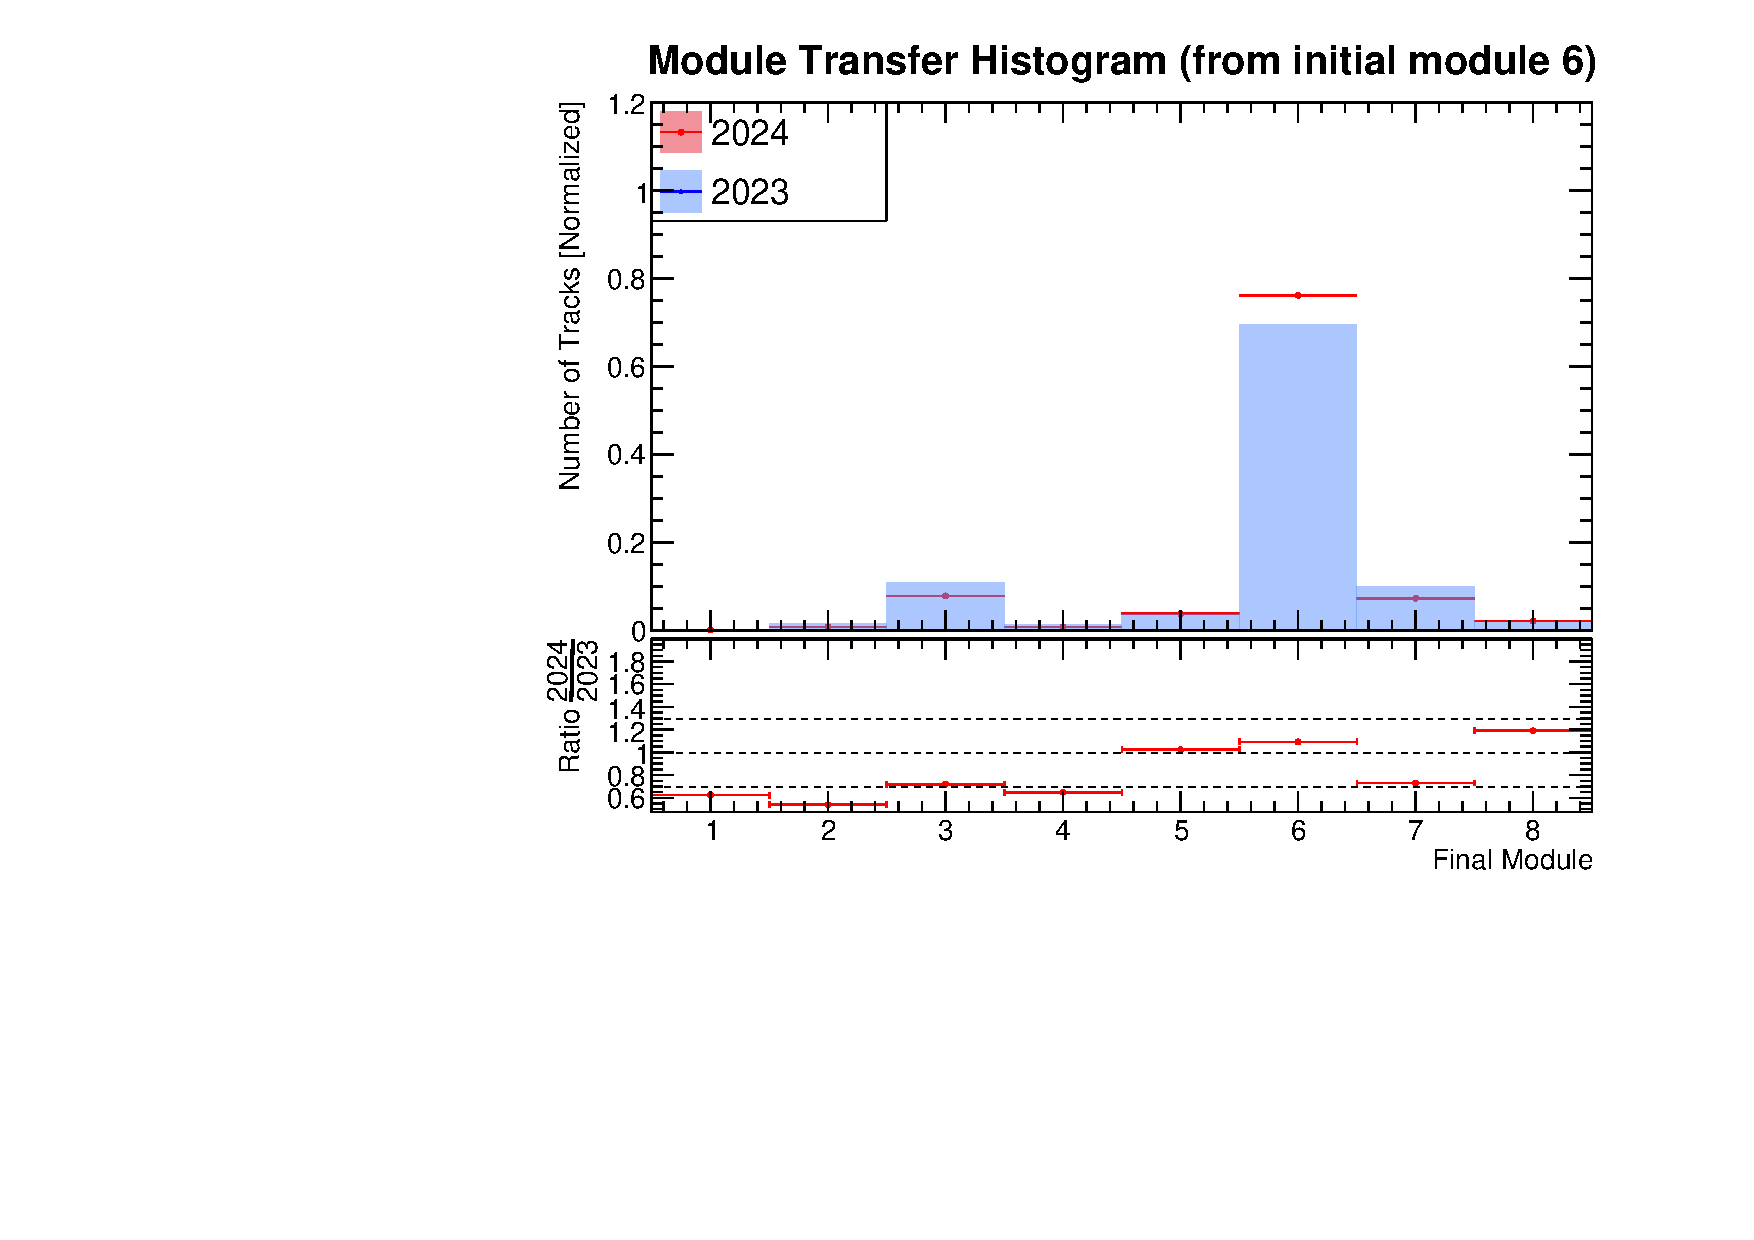
\includegraphics[width=\linewidth]{./ModuleLevelPlots/final_module_from_st0_module6.pdf}
        \end{subfigure}

        \begin{subfigure}[t]{0.49\linewidth}
            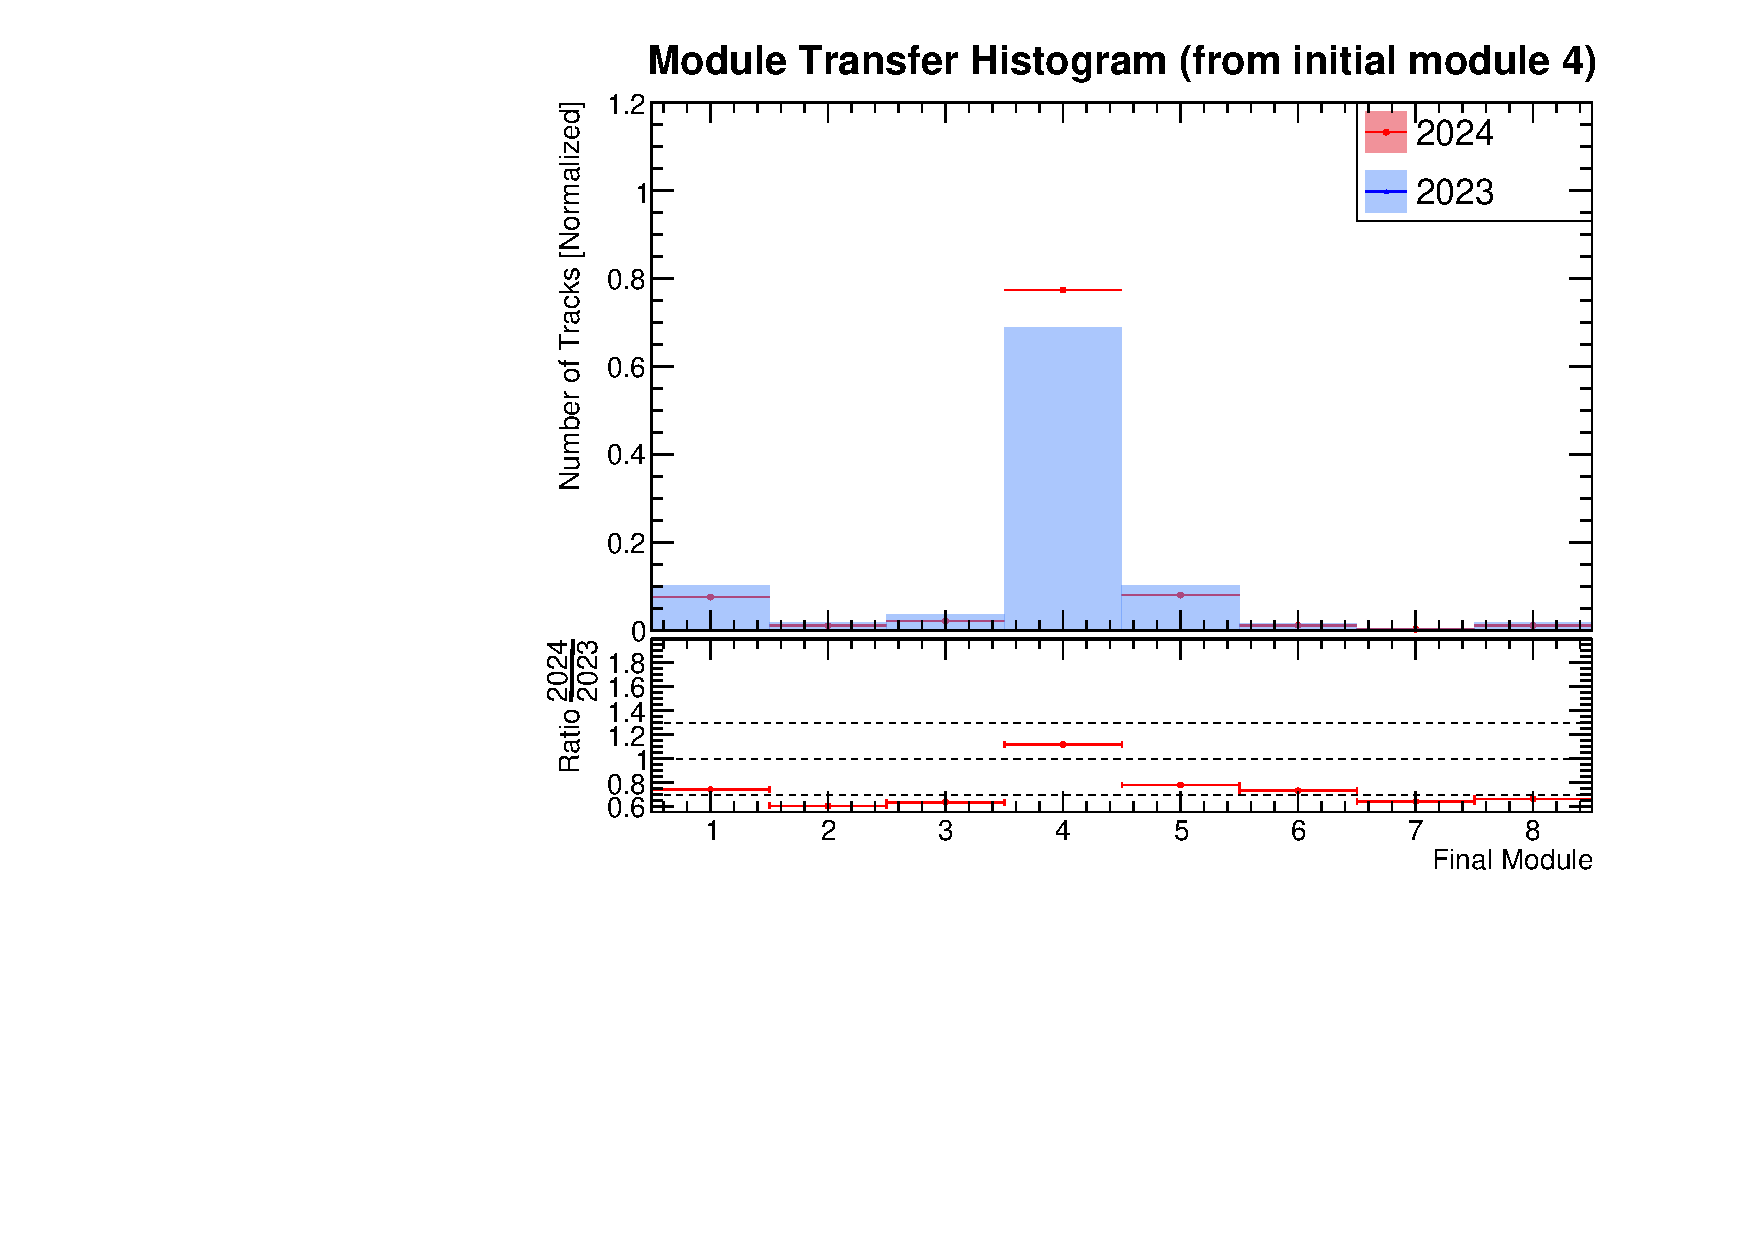
\includegraphics[width=\linewidth]{./ModuleLevelPlots/final_module_from_st0_module4.pdf}
        \end{subfigure}
        \begin{subfigure}[t]{0.49\linewidth}
            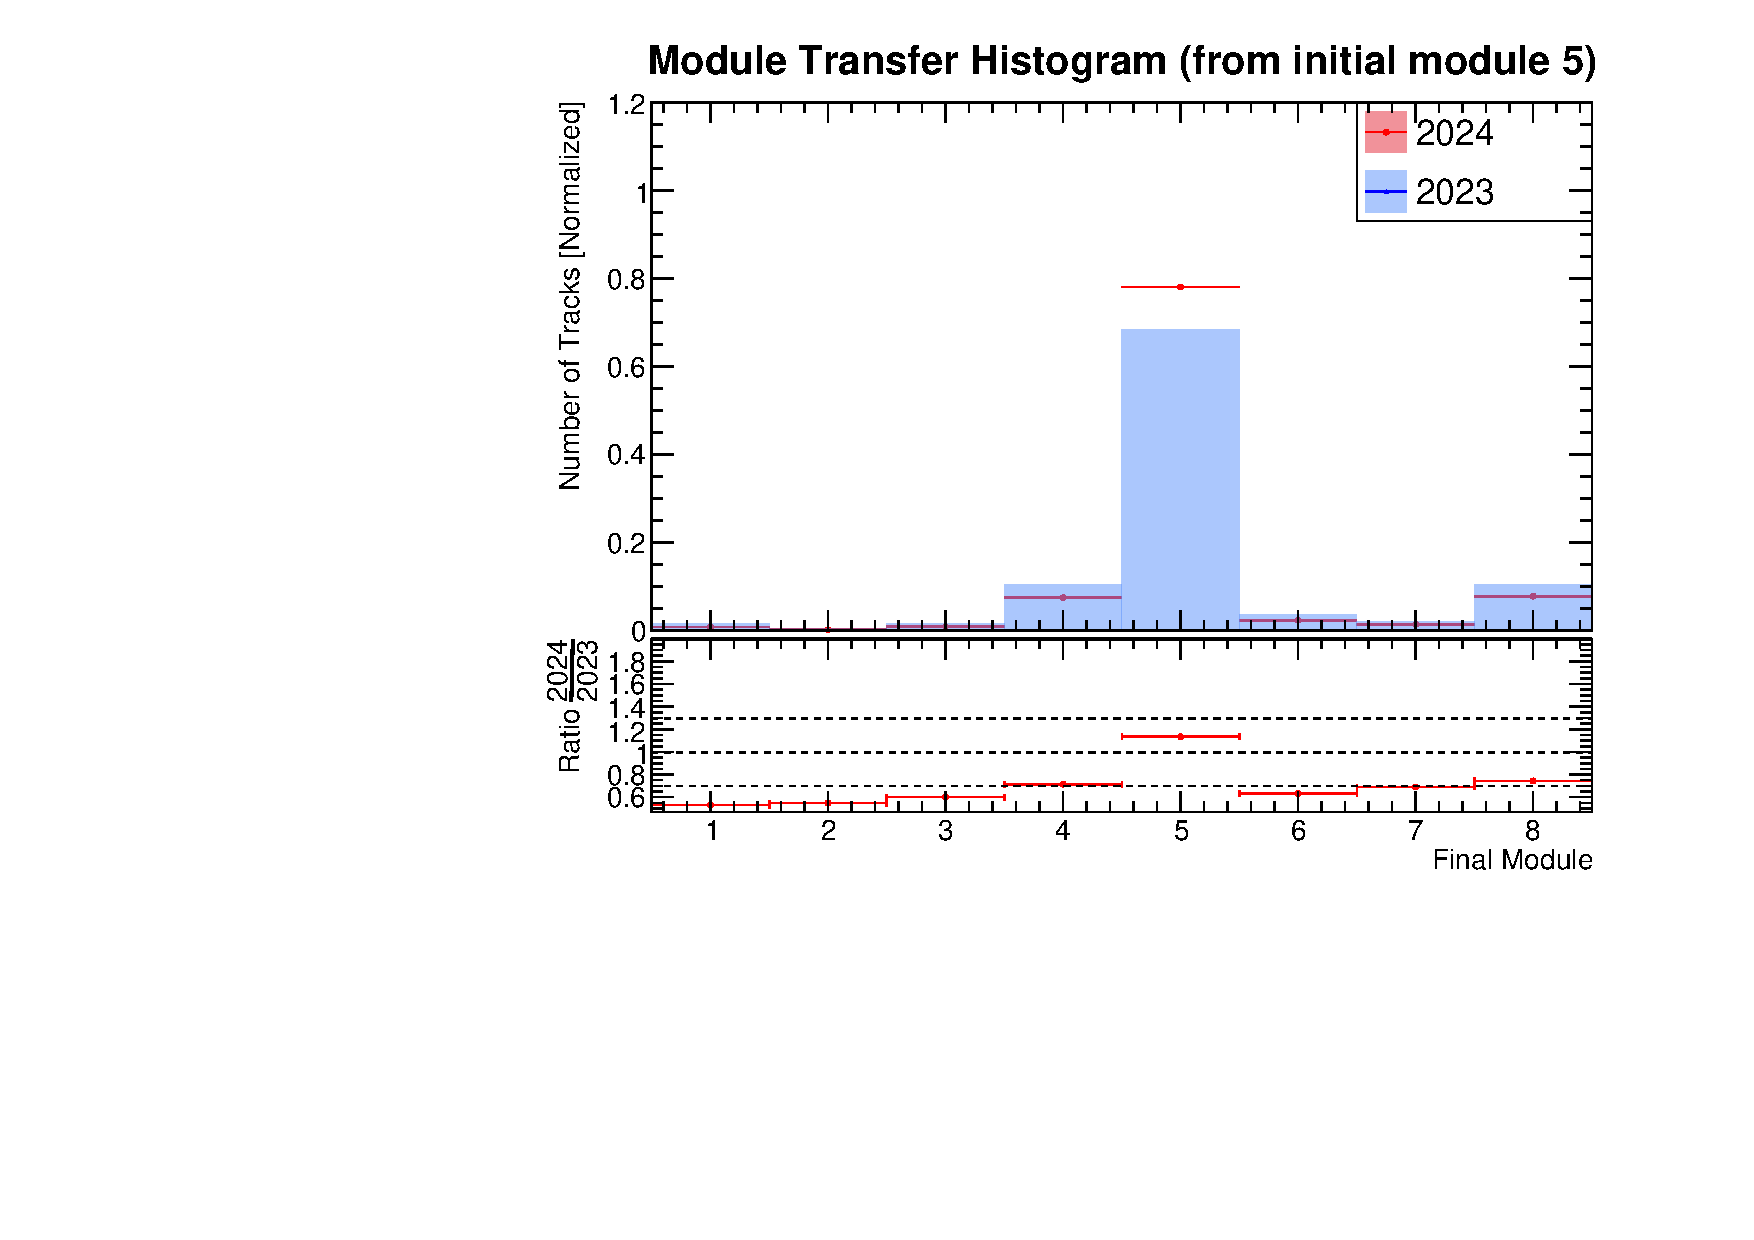
\includegraphics[width=\linewidth]{./ModuleLevelPlots/final_module_from_st0_module5.pdf}
        \end{subfigure}
    \end{figure}
\end{frame}

% \section{Track Parameters Modulewise}    

\begin{frame}{Modulewise Track Parameters}
    
    Recap of the Track Parameters:
    \begin{itemize}
        \item Number of longTracks
        \item Track Charge
        \item Track Chi2 
        \item Track Chi2perDoF
        \item Track nDoF
        \item Track In Station [SKIP]
        \item Track nLayers
        \item Track Propagation Error [SKIP]
    \end{itemize}
    \vspace{0.3 cm}
    \small{    
    Note: Unfortunately, 8 modules across 2 year = 16 Histograms \\
    An year wise for each module would be too long.
    So we do a module level comparison, year wise plots available in the backup.
    }
    % \begin{itemize}
    %     \item Hard to visualize, so we do a module level comparison
    %     \item More detailed plots available in the backup/repo
    % \end{itemize}
\end{frame}




\newcommand{\makemodulewiseframes}[2]{
    \begin{frame}{#2}
        \newcommand{\colname}{#1}
        \begin{figure}
            \centering
            \begin{subfigure}[t]{0.49\linewidth}
                \includegraphics[width=\linewidth]{./ModuleLevelPlots/\colname_st0_module1.pdf}
            \end{subfigure}
            \begin{subfigure}[t]{0.49\linewidth}
                \includegraphics[width=\linewidth]{./ModuleLevelPlots/\colname_st0_module8.pdf}
            \end{subfigure}
    
            \begin{subfigure}[t]{0.49\linewidth}
                \includegraphics[width=\linewidth]{./ModuleLevelPlots/\colname_st0_module2.pdf}
            \end{subfigure}
            \begin{subfigure}[t]{0.49\linewidth}
                \includegraphics[width=\linewidth]{./ModuleLevelPlots/\colname_st0_module7.pdf}
            \end{subfigure}
        \end{figure}
    \end{frame}
    \begin{frame}{#2 [Contd.]}
        \newcommand{\colname}{#1}
        \begin{figure}
            \centering
            \begin{subfigure}[t]{0.49\linewidth}
                \includegraphics[width=\linewidth]{./ModuleLevelPlots/\colname_st0_module3.pdf}
            \end{subfigure}
            \begin{subfigure}[t]{0.49\linewidth}
                \includegraphics[width=\linewidth]{./ModuleLevelPlots/\colname_st0_module6.pdf}
            \end{subfigure}
    
            \begin{subfigure}[t]{0.49\linewidth}
                \includegraphics[width=\linewidth]{./ModuleLevelPlots/\colname_st0_module4.pdf}
            \end{subfigure}
            \begin{subfigure}[t]{0.49\linewidth}
                \includegraphics[width=\linewidth]{./ModuleLevelPlots/\colname_st0_module5.pdf}
            \end{subfigure}
        \end{figure}
    \end{frame}

}



\makemodulewiseframes{longTracks}{Distribution longTracks Modulewise}
\begin{frame}{Distribution longTracks Modulewise}
    \newcommand{\colname}{longTracks}
    \begin{columns}
        \begin{column}{0.6\linewidth}
            \begin{figure}
                \centering
                \includegraphics[width=\linewidth]{./ModuleLevelPlots/\colname_st0_2023.pdf}
            \end{figure}
        \end{column}
        \begin{column}{0.6\linewidth}
            \begin{figure}
                \centering
                \includegraphics[width=\linewidth]{./ModuleLevelPlots/\colname_st0_2024.pdf}
            \end{figure}
        \end{column}
    \end{columns}
    \begin{itemize}
        \item 2024 has more events in the tail
        \item Seem to form two layers with 
        \begin{itemize}
            \item Modules 2,7,8 having lower long tracks [highly pronounced in bin2]
            \item Seem to merge for higher bins
        \end{itemize}
    \end{itemize}
\end{frame}

\makemodulewiseframes{Track_charge}{Distribution of Track Charge Modulewise}
\begin{frame}{Distribution Track Charge Modulewise}
    \newcommand{\colname}{Track_charge}
    \begin{columns}
        \begin{column}{0.6\linewidth}
            \begin{figure}
                \centering
                \includegraphics[width=\linewidth]{./ModuleLevelPlots/\colname_st0_2023.pdf}
            \end{figure}
        \end{column}
        \begin{column}{0.6\linewidth}
            \begin{figure}
                \centering
                \includegraphics[width=\linewidth]{./ModuleLevelPlots/\colname_st0_2024.pdf}
            \end{figure}
        \end{column}
    \end{columns}

    \begin{itemize}
        \small
        \item 2023 has more negatively charged tracks
        \item In 2023 Module 1,2 seem to get more positively charged tracks[Why?]
        \item In 2024 Module 3,6,7,5 seem to get more positively charged tracks
        \begin{itemize}
            \item Suggests, positive tracks coming in from the bottom right?
        \end{itemize}
    \end{itemize}
\end{frame}

\makemodulewiseframes{Track_Chi2}{Track Chi2 Modulewise}
\begin{frame}{Track Chi2 Modulewise}
    \newcommand{\colname}{Track_Chi2}
    \begin{columns}
        \begin{column}{0.6\linewidth}
            \begin{figure}
                \centering
                \includegraphics[width=\linewidth]{./ModuleLevelPlots/\colname_st0_2023.pdf}
            \end{figure}
        \end{column}
        \begin{column}{0.6\linewidth}
            \begin{figure}
                \centering
                \includegraphics[width=\linewidth]{./ModuleLevelPlots/\colname_st0_2024.pdf}
            \end{figure}
        \end{column}
    \end{columns}

    \begin{itemize}
        \small
        \item Better Agreement in 2024 
        \item Module 2 shows higher Track Chi2 in 2023
    \end{itemize}
\end{frame}

\makemodulewiseframes{Track_nDoF}{Track Degrees of Freedom Modulewise}
\begin{frame}{Track Degrees of Freedom Modulewise}
    \newcommand{\colname}{Track_nDoF}
    \begin{columns}
        \begin{column}{0.6\linewidth}
            \begin{figure}
                \centering
                \includegraphics[width=\linewidth]{./ModuleLevelPlots/\colname_st0_2023.pdf}
            \end{figure}
        \end{column}
        \begin{column}{0.6\linewidth}
            \begin{figure}
                \centering
                \includegraphics[width=\linewidth]{./ModuleLevelPlots/\colname_st0_2024.pdf}
            \end{figure}
        \end{column}
    \end{columns}

    \begin{itemize}
        \small
        \item Module 2 has higher nDoF in 2024
        \item Track NDoF split into two groups
        \begin{itemize}
            \item Higher nDoF Modules : 2, 1, 8, 7 [Modules with y $\geq$ 0]
            \item Lower nDoF Modules \ : 3, 4, 5, 6  [Modules with y $\leq$ 0]
        \end{itemize}
    \end{itemize}
\end{frame}

\makemodulewiseframes{Track_Chi2perDoF}{Track Chi2perDoF Modulewise}
\begin{frame}{Track Chi2perDoF Modulewise}
    \newcommand{\colname}{Track_Chi2perDoF}
    \begin{columns}
        \begin{column}{0.6\linewidth}
            \begin{figure}
                \centering
                \includegraphics[width=\linewidth]{./ModuleLevelPlots/\colname_st0_2023.pdf}
            \end{figure}
        \end{column}
        \begin{column}{0.6\linewidth}
            \begin{figure}
                \centering
                \includegraphics[width=\linewidth]{./ModuleLevelPlots/\colname_st0_2024.pdf}
            \end{figure}
        \end{column}
    \end{columns}

    \begin{itemize}
        \small
        \item In 2023, the Track Chi2 seem to split into two groups
        \begin{itemize}
            \item Higher Chi2 Modules : 2, 1, 8, 7 [Modules with y $\geq$ 0]
            \item Lower Chi2 Modules \ : 3, 4, 5, 6  [Modules with y $\leq$ 0]
        \end{itemize}
    \end{itemize}
\end{frame}

\makemodulewiseframes{Track_nLayers}{Distribution of Track\_nLayers Modulewise}
\begin{frame}{Distribution of Track\_nLayers Modulewise}
    \newcommand{\colname}{Track_nLayers}
    \begin{columns}
        \begin{column}{0.6\linewidth}
            \begin{figure}
                \centering
                \includegraphics[width=\linewidth]{./ModuleLevelPlots/\colname_st0_2023.pdf}
            \end{figure}
        \end{column}
        \begin{column}{0.6\linewidth}
            \begin{figure}
                \centering
                \includegraphics[width=\linewidth]{./ModuleLevelPlots/\colname_st0_2024.pdf}
            \end{figure}
        \end{column}
    \end{columns}

    \begin{itemize}
        \small
        \item Again seem to split into two groups
        \begin{itemize}
            \item Higher nLayer Modules : 2, 1, 8, 7 [Modules with y $\geq$ 0]
            \item Lower nLayer Modules \ : 3, 4, 5, 6  [Modules with y $\leq$ 0]
        \end{itemize}
    \end{itemize}
\end{frame}


% \makebinnedframes{Track_p0}{Distribution of Track Momentum Modulewise}
\begin{frame}{Distribution of Track Momentum Modulewise}
    TODO..
\end{frame}


\begin{frame}{Recap of 2024 Runs Splits}
    \begin{itemize}
        \item Due to the higher backgrounds FaserNu had to be replaced every 10 fb$^-1$.
        \item The replacement schedule was as follows
    \end{itemize}
    \begin{table}[h!]
        \begin{tabular}{|l|c|c|c|}
            \hline
            \textbf{Box}  & \textbf{Installed} & \textbf{Removed} & \textbf{Lumi (ifb)} \\ \hline
            F241          & 20/3               & 6/5              & 11.6                \\ \hline
            Tungsten only & 6/5                & 12/6             & 18.5                \\ \hline
            F242          & 12/6               & 8/7              & 9.9                 \\ \hline
            CaloNu        & 10/7               & 4/10             & 69.8                \\ \hline
            F243          & 4/10               & 22/10            & 11.9                \\ \hline
        \end{tabular}
        \caption{Replacement Schedule [Source: \href{https://indico.cern.ch/event/1350805/contributions/5686417/attachments/2963344/5212652/FASER-GeneralMtg-8.11.24.pdf}{FASER General Meeting 8.11.24}]}
    \end{table}
	\vspace{-0.5cm}
    \begin{itemize}
        \item The runs are split into categories based on the above schedule
        % \item Allowed a construction of Yield plots for each category, NEvents/Lumi (Top) and NTracks/Lumi (Bottom)
    \end{itemize}
    \scriptsize{Note: Detailed Calculation of Run Numbers can be found here [Link to Sheet]}
\end{frame}

\begin{frame}{Issues with BCID}
	\begin{itemize}
		\item Reminder that the 2024 data is split into as p0011 and p0012
		\item The p0011 data has issues with the BCID makes the distanceToCollidingBCID unreliable
		\item But unfortunately, p0011 data is more than 55\% of the 2024 data
		\item Following plots apply the BCID cut only on the 2023 data and the p0012 data. 
	\end{itemize}
	\begin{figure}
		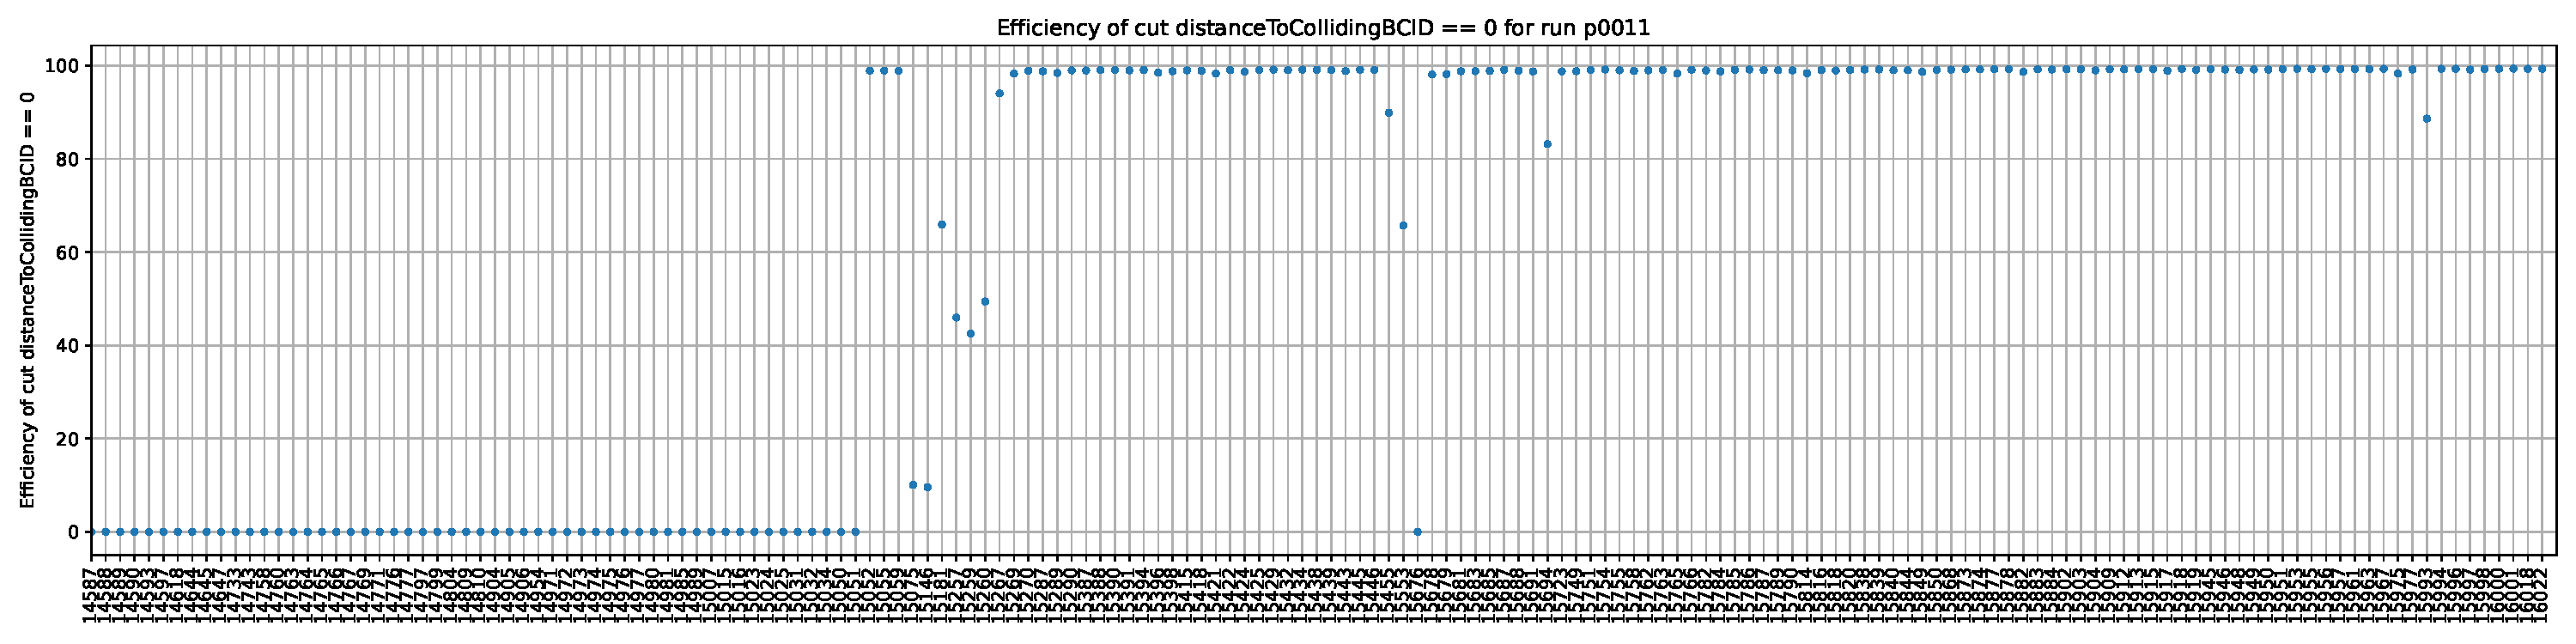
\includegraphics[width=\linewidth]{./assets/BCIDEfficiency_p0011.pdf}
		\caption{Efficiency of the BCID cut on the p0011 data}
	\end{figure}

\end{frame}

\begin{frame}{Yield Plots for F241-2024}
	\begin{figure}
		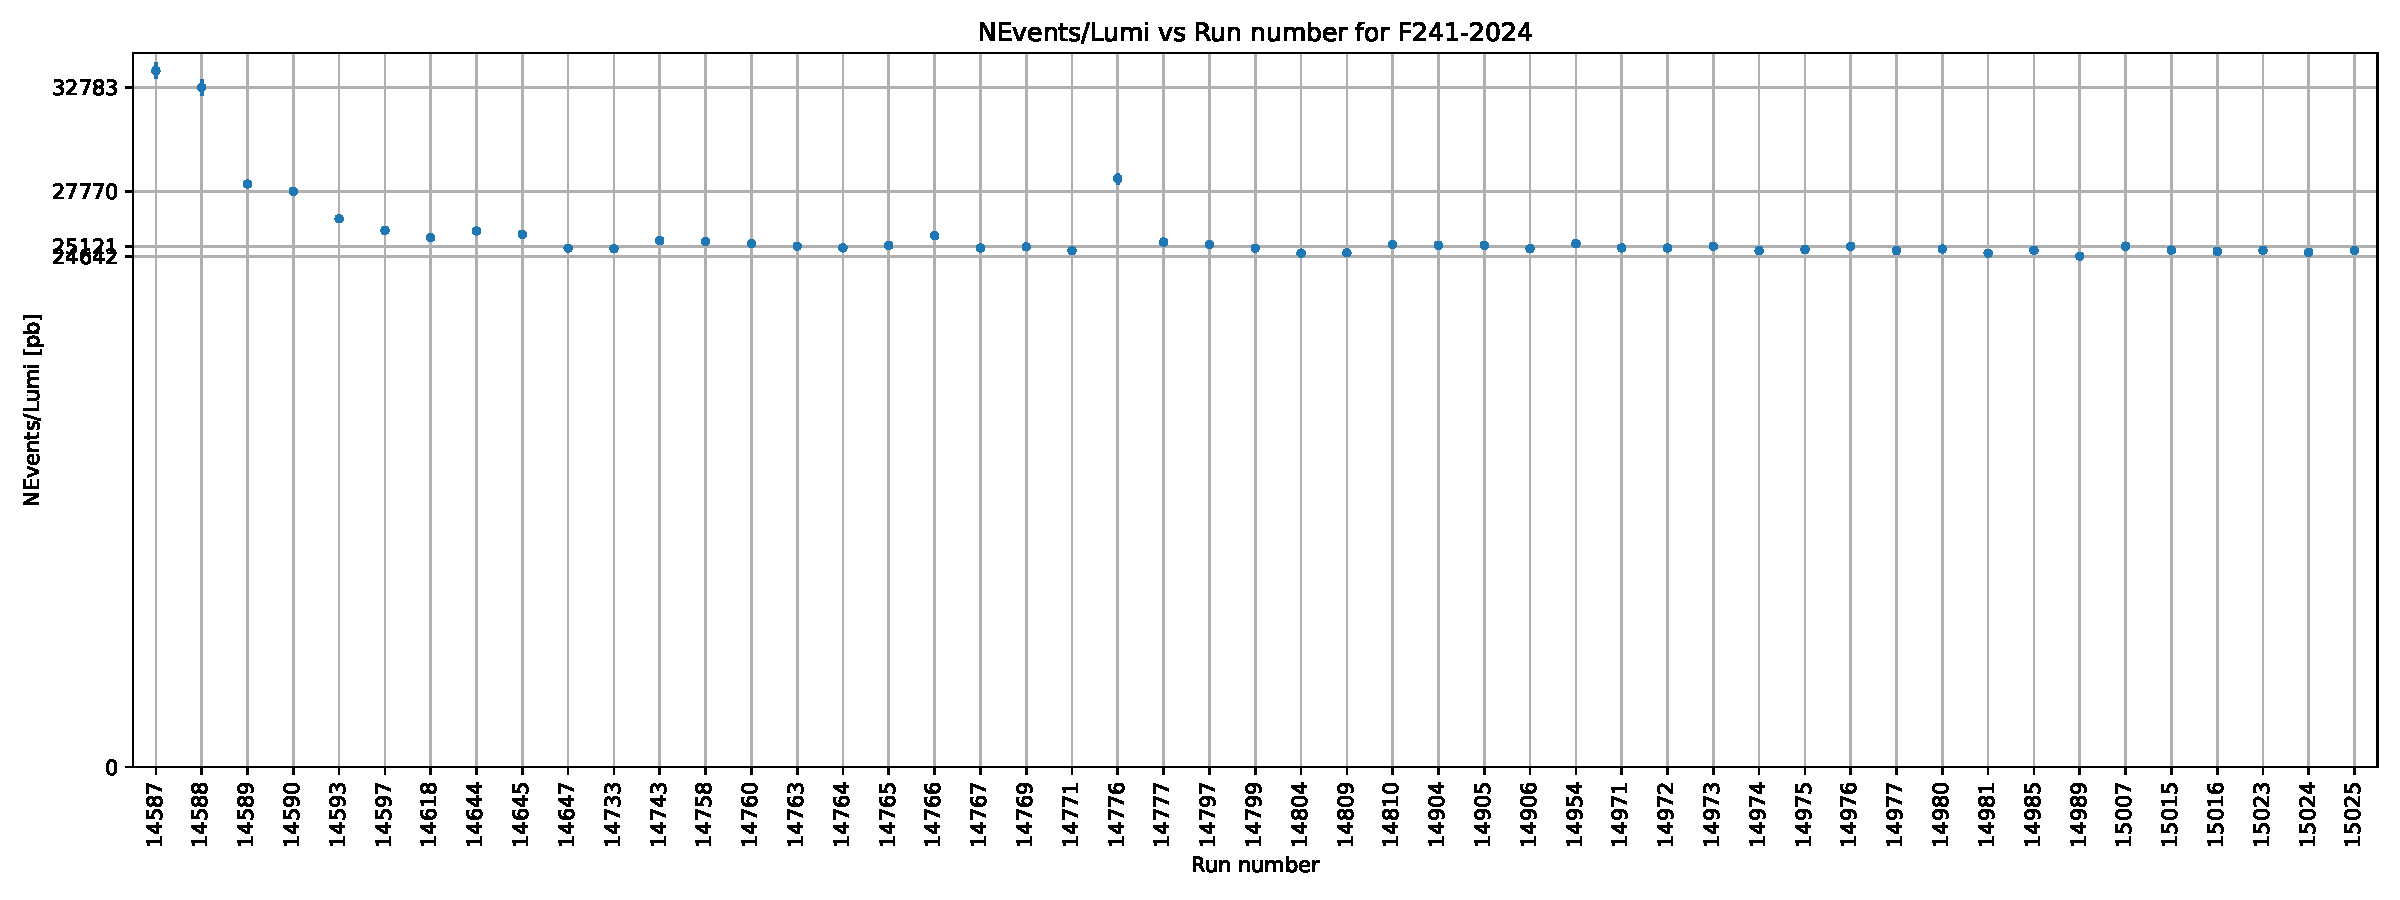
\includegraphics[height=0.4\textheight]{RunwisePlots/F241-2024_NEventsbyLumi.pdf}
	\end{figure}
	\begin{figure}
		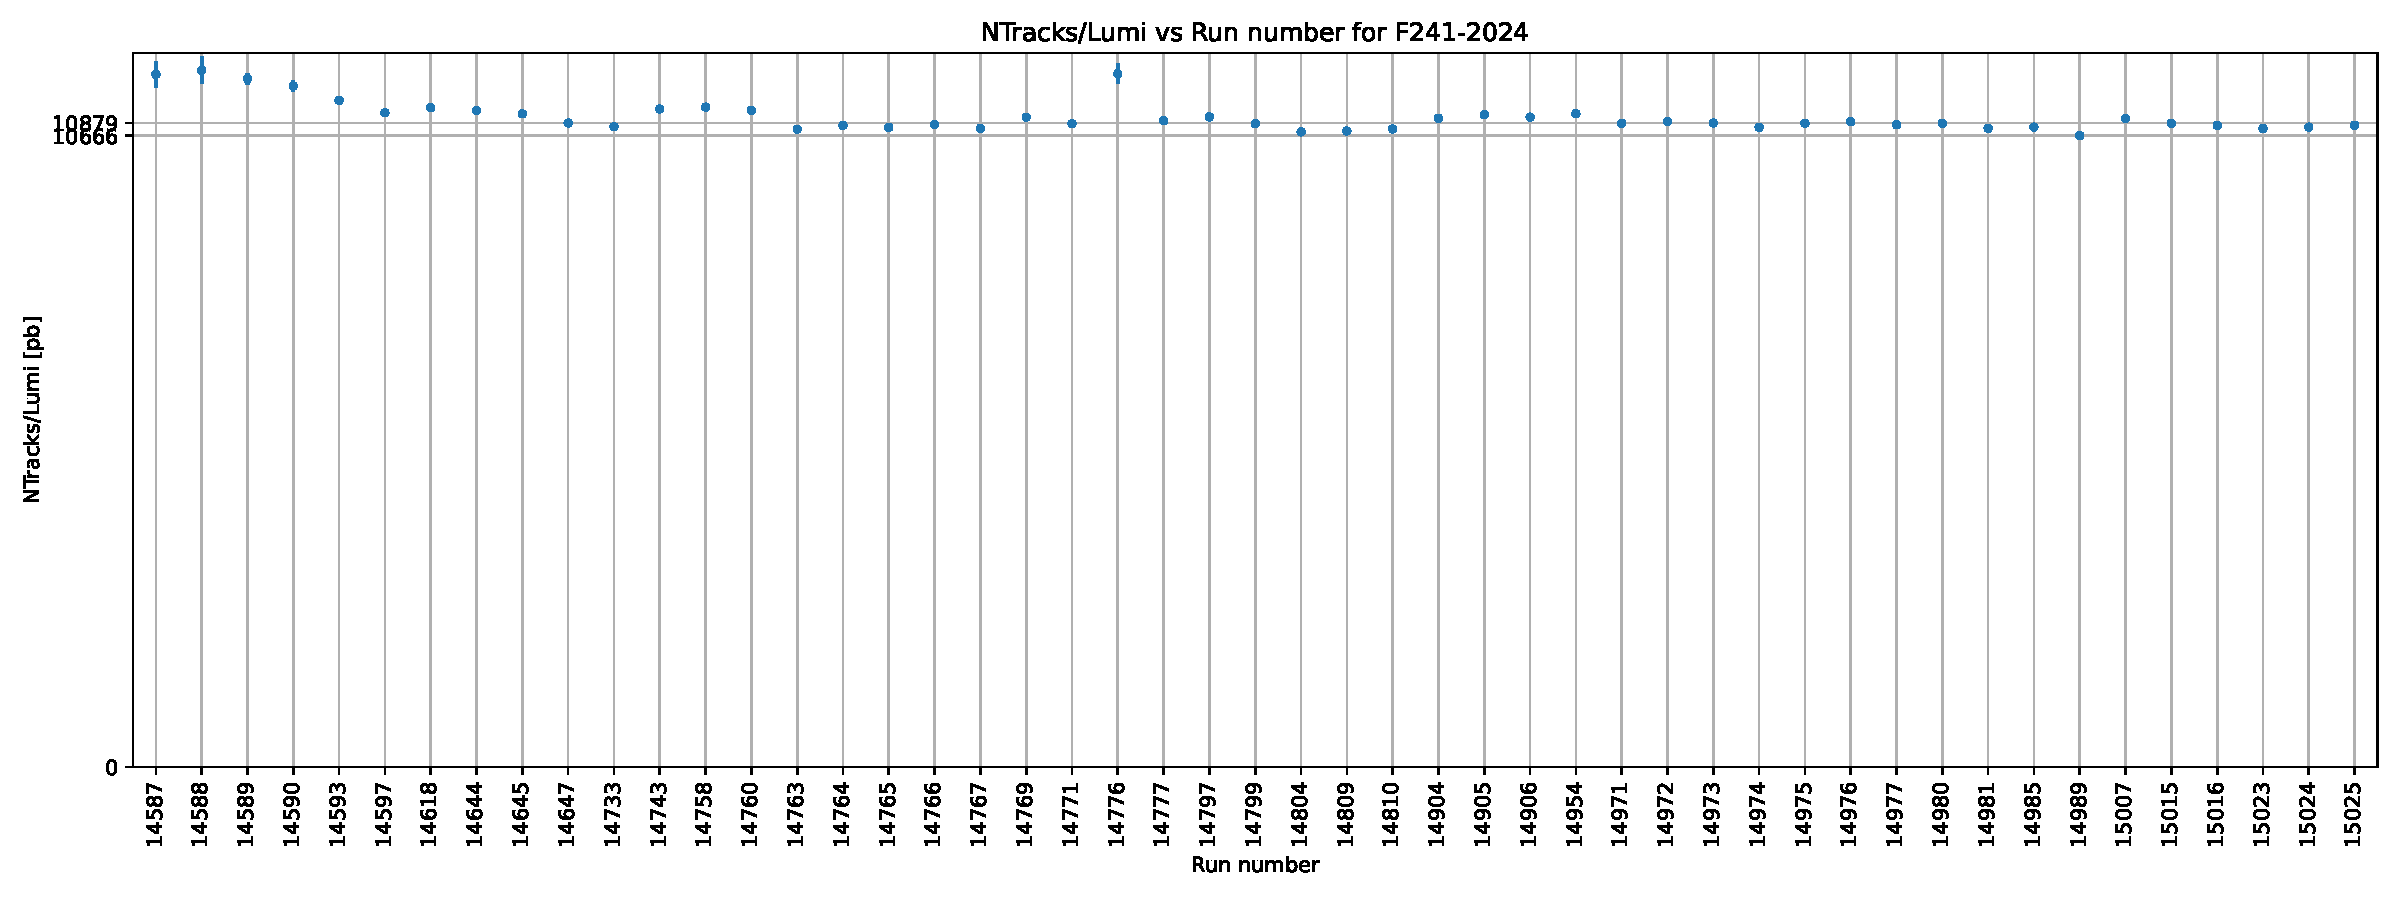
\includegraphics[height=0.4\textheight]{RunwisePlots/F241-2024_NTracksbyLumi.pdf}
	\end{figure}
\end{frame}

\begin{frame}{Yield Plots for Tungsten-2024}
	\begin{figure}
		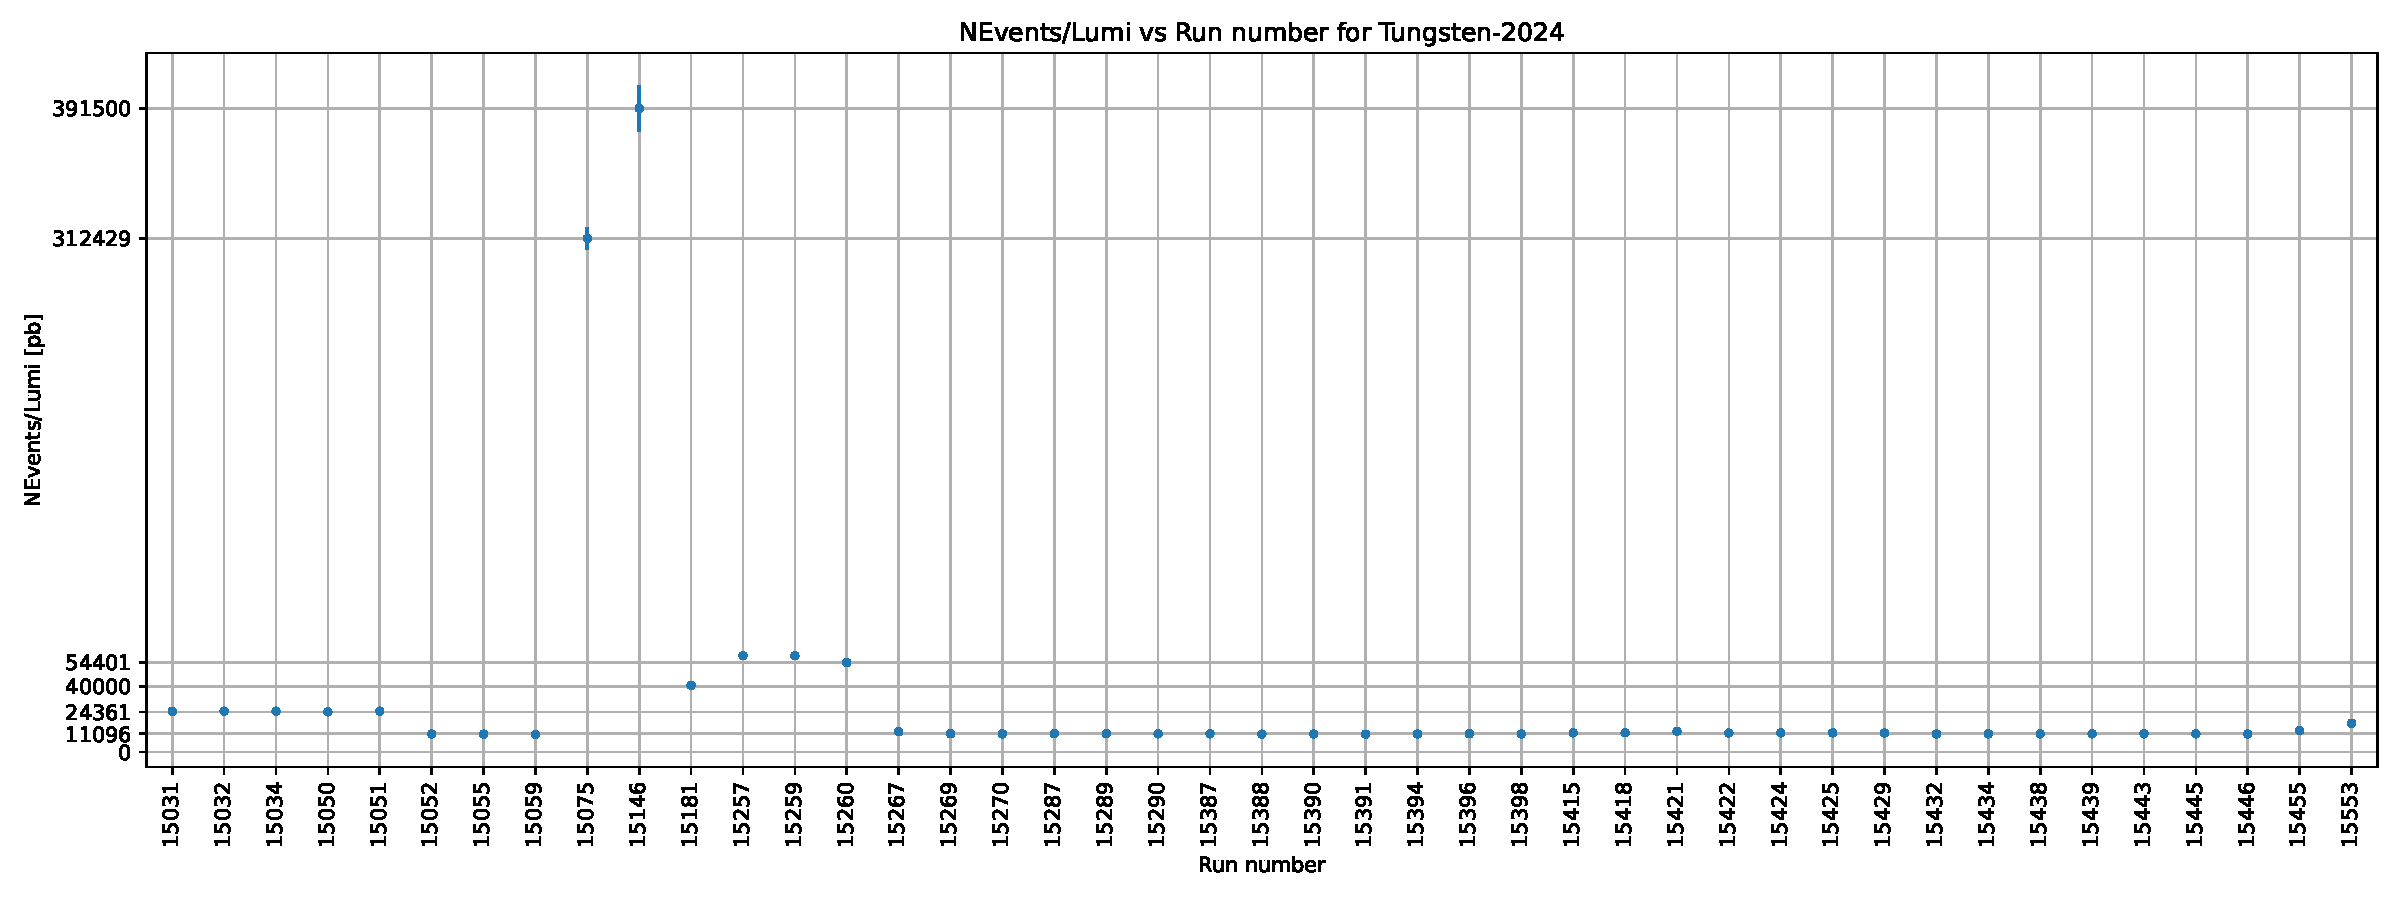
\includegraphics[height=0.4\textheight]{RunwisePlots/Tungsten-2024_NEventsbyLumi.pdf}
	\end{figure}
	\begin{figure}
		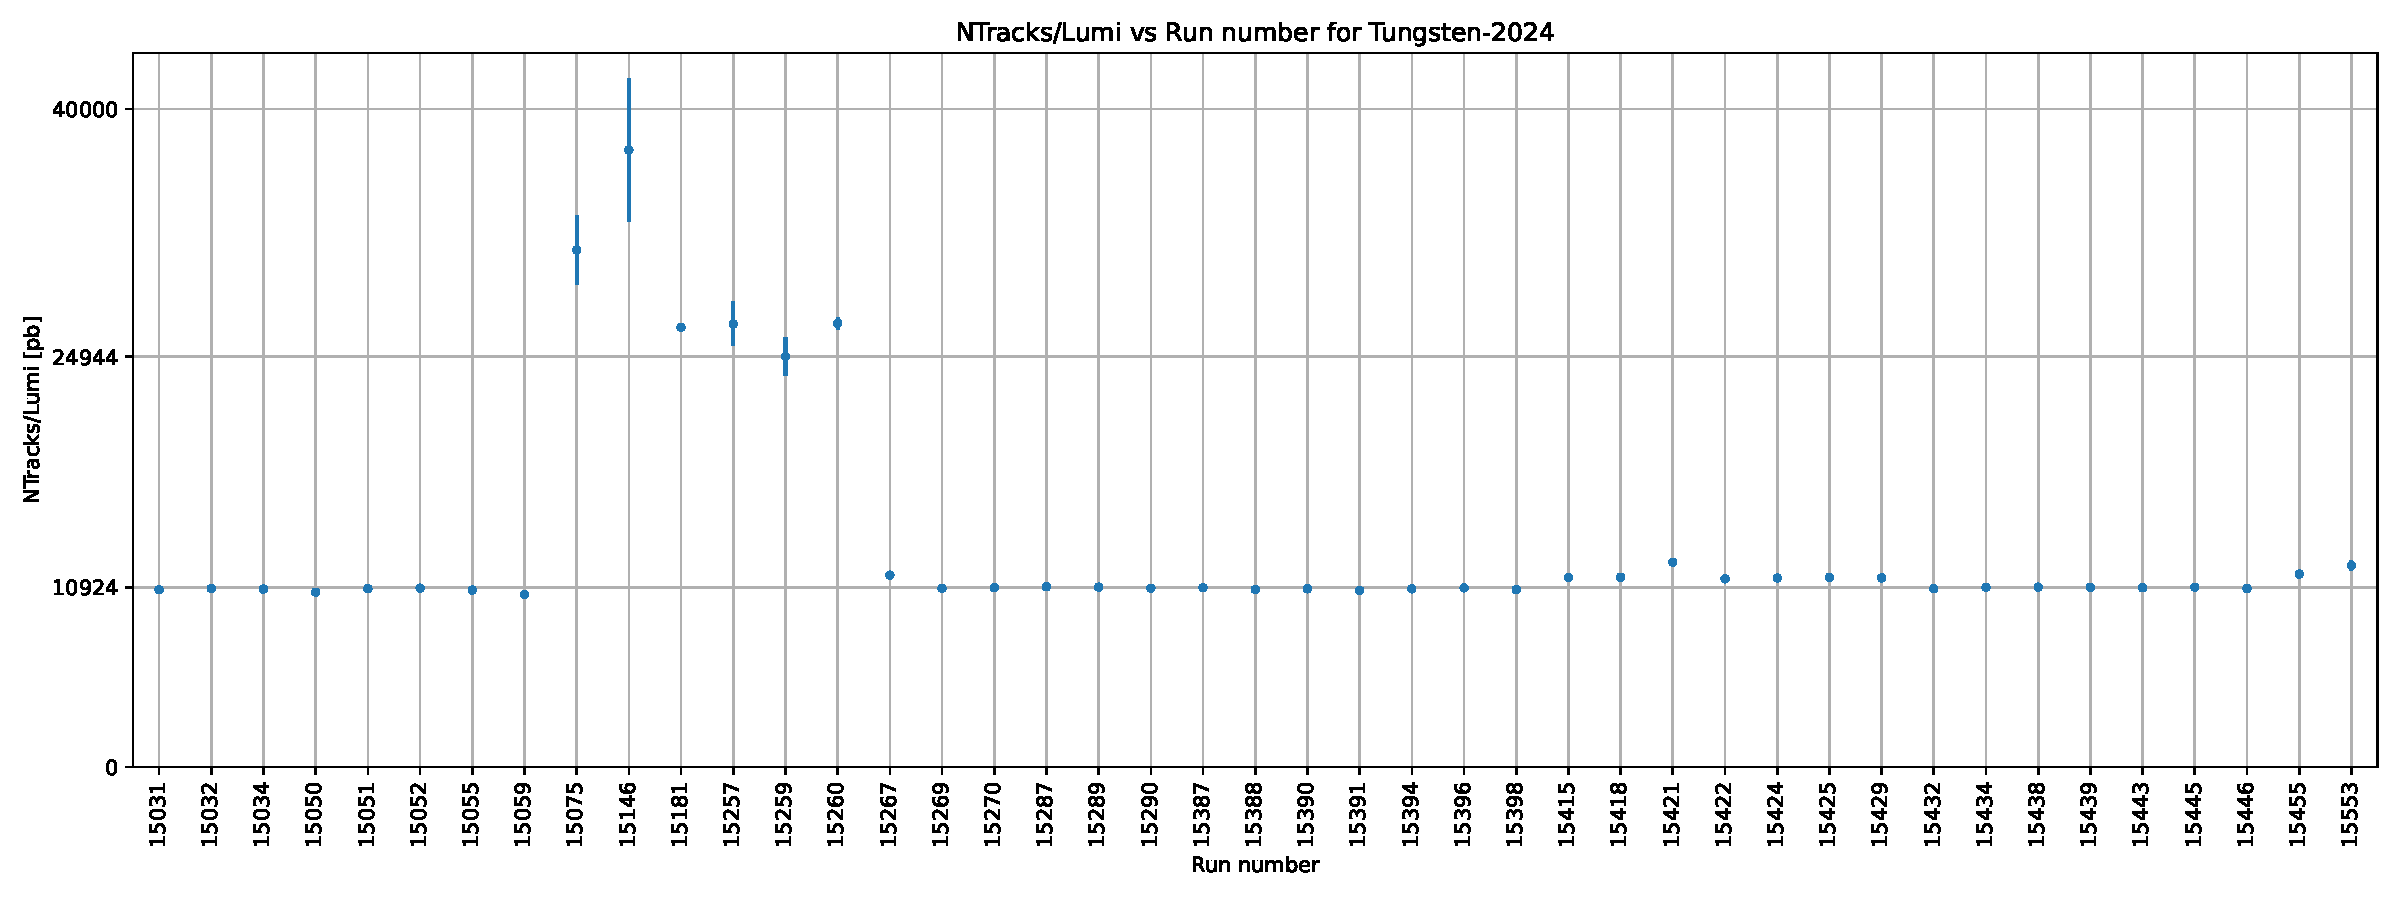
\includegraphics[height=0.4\textheight]{RunwisePlots/Tungsten-2024_NTracksbyLumi.pdf}
	\end{figure}
\end{frame}

\begin{frame}{Yield Plots for F242-2024}
	\begin{figure}
		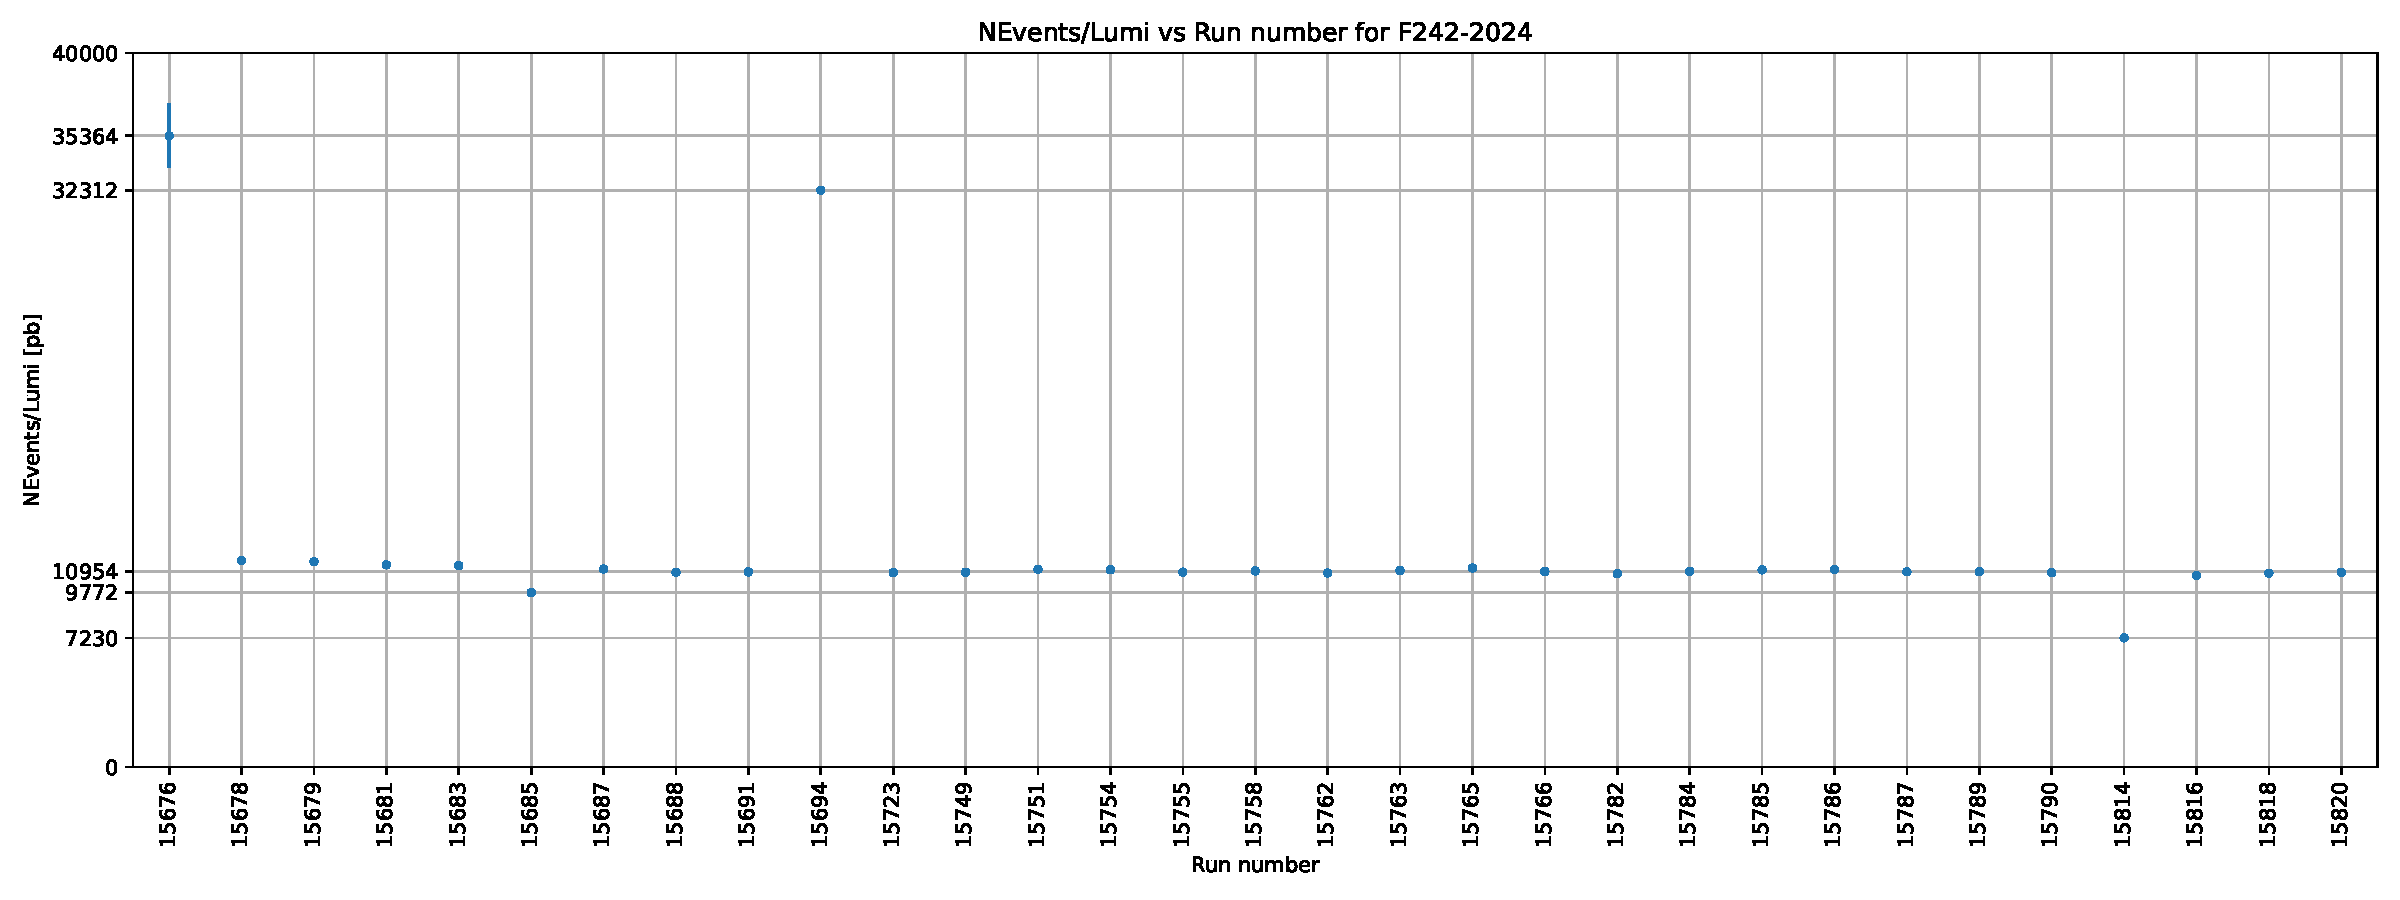
\includegraphics[height=0.4\textheight]{RunwisePlots/F242-2024_NEventsbyLumi.pdf}
	\end{figure}
	\begin{figure}
		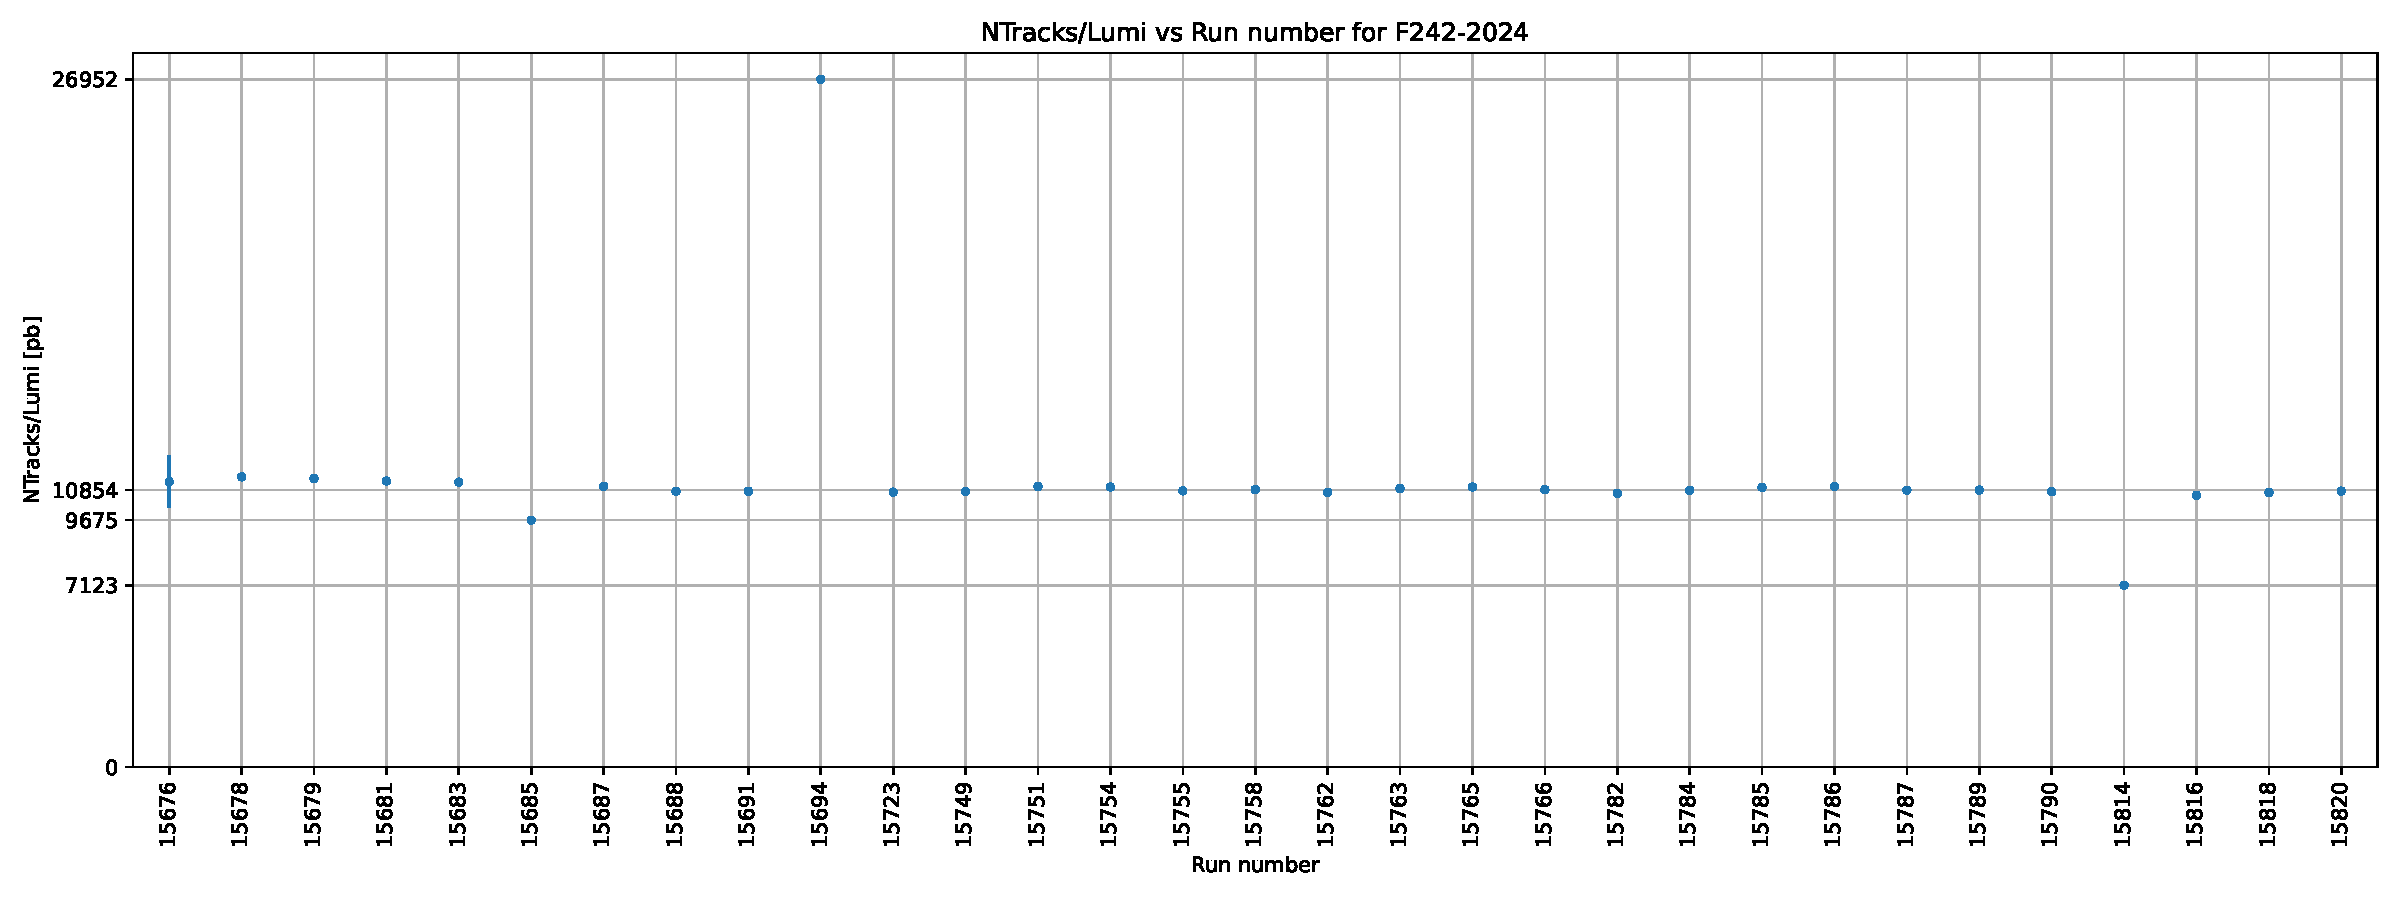
\includegraphics[height=0.4\textheight]{RunwisePlots/F242-2024_NTracksbyLumi.pdf}
	\end{figure}
\end{frame}

\begin{frame}{Yield Plots for CaloNu-2024}
	\begin{figure}
		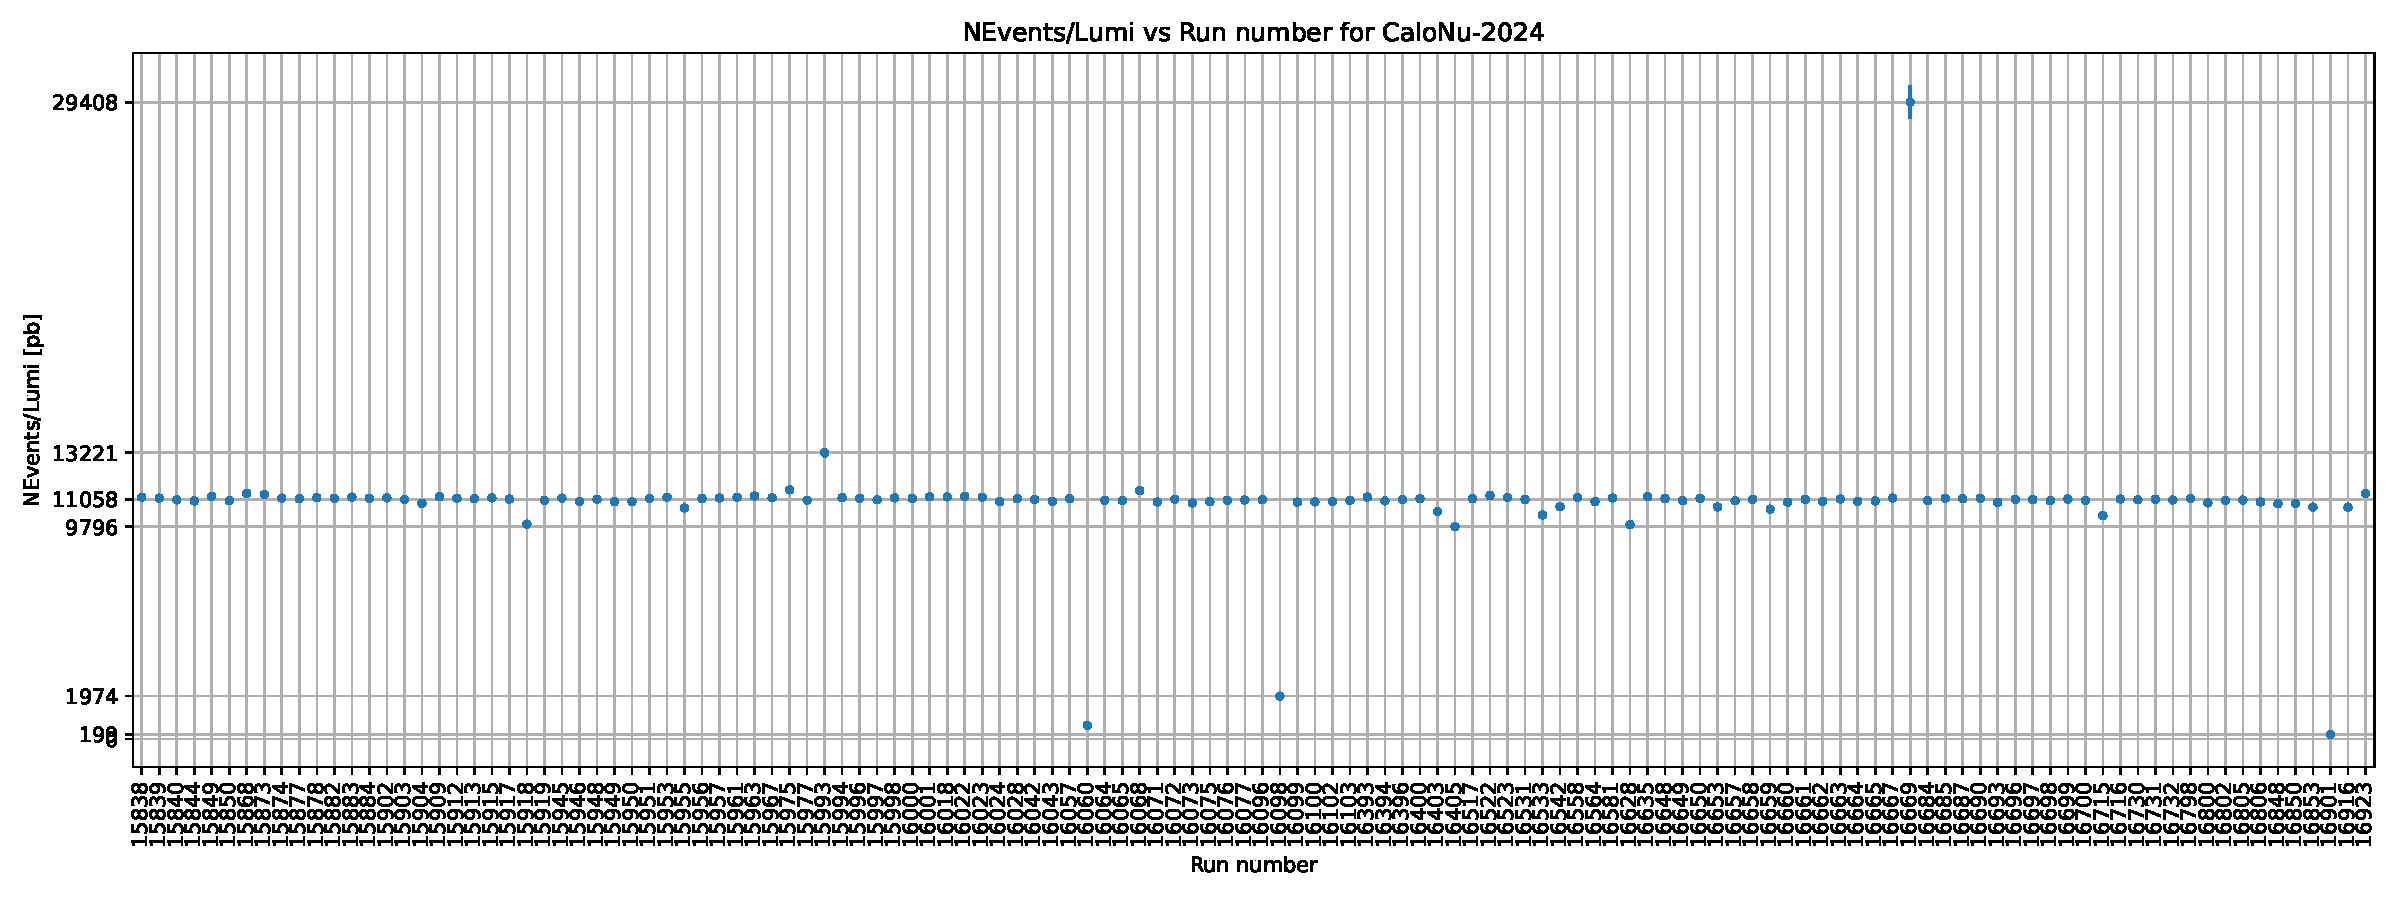
\includegraphics[height=0.4\textheight]{RunwisePlots/CaloNu-2024_NEventsbyLumi.pdf}
	\end{figure}
	\begin{figure}
		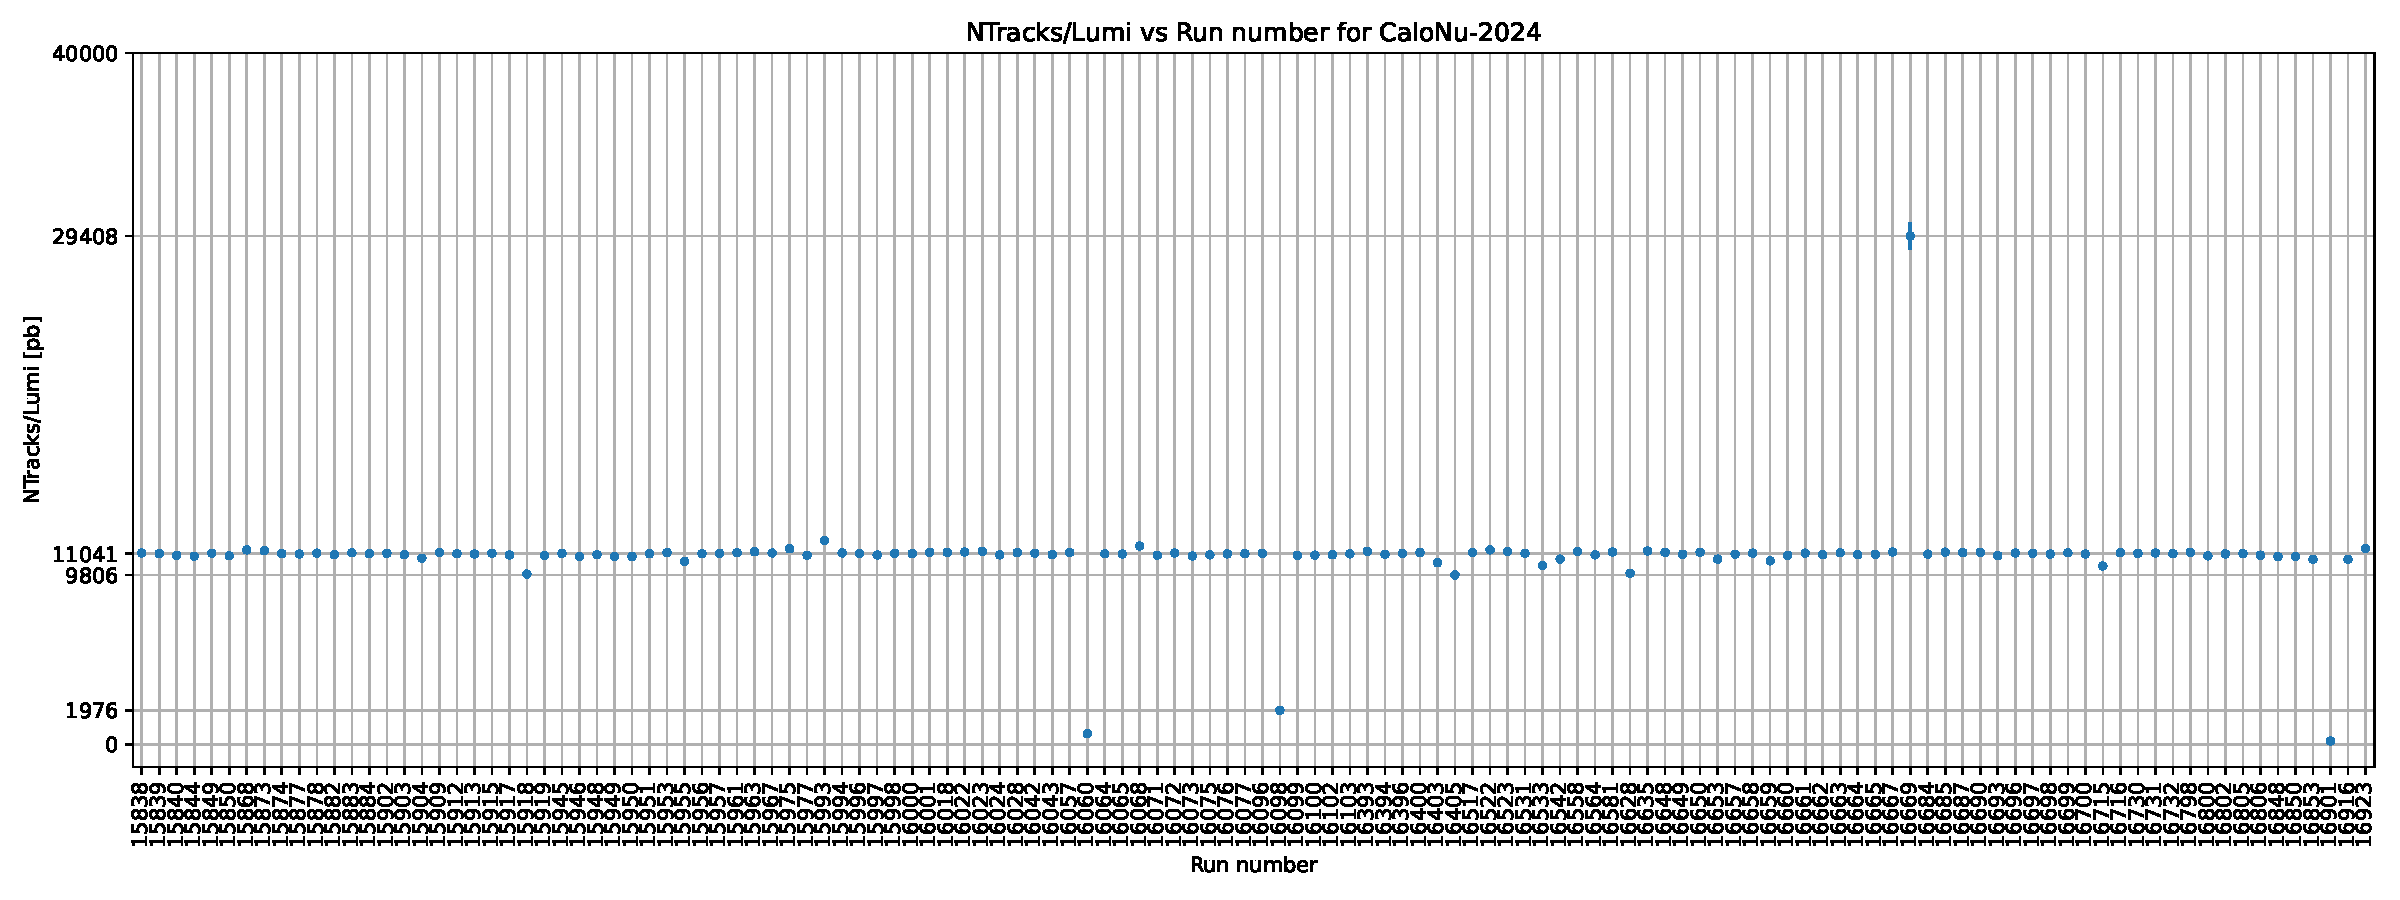
\includegraphics[height=0.4\textheight]{RunwisePlots/CaloNu-2024_NTracksbyLumi.pdf}
	\end{figure}
\end{frame}

\begin{frame}{Yield Plots for F243-2024}
	\begin{figure}
		\includegraphics[height=0.4\textheight]{RunwisePlots/F243-2024_NEventsbyLumi.pdf}
	\end{figure}
	\begin{figure}
		\includegraphics[height=0.4\textheight]{RunwisePlots/F243-2024_NTracksbyLumi.pdf}
	\end{figure}
\end{frame}

\begin{frame}{Median Yeilds across Runs}
	\begin{figure}
		\includegraphics[width=\linewidth]{./RunwisePlots/MedianYieldsPhase.pdf}
	\end{figure}
	\vspace{-0.5cm}
	\begin{itemize}
		\item Possible anomaly in the F241 data?
	\end{itemize}
\end{frame}

\begin{frame}{Distribution of Track Parameters across Runs}
	\begin{center}
		Excellent agreement of variables across runs !
	\end{center}
	
\end{frame}


\begin{frame}{Distribution of Track X0 across 2024 runs}
	\begin{figure}
		\includegraphics[width=\linewidth]{./RunwisePlots/Track_x0_runwise.pdf}
	\end{figure}
\end{frame}
\begin{frame}{Distribution of Track Y0 across runs}
	\begin{figure}
		\includegraphics[width=\linewidth]{./RunwisePlots/Track_y0_runwise.pdf}
	\end{figure}
\end{frame}

\begin{frame}{Distribution of Track ThetaX0 across 2024 runs}
	\begin{figure}
		\includegraphics[width=\linewidth]{./RunwisePlots/Track_ThetaX_0_runwise.pdf}
	\end{figure}
\end{frame}
\begin{frame}{Distribution of Track ThetaY0 across runs}
	\begin{figure}
		\includegraphics[width=\linewidth]{./RunwisePlots/Track_ThetaY_0_runwise.pdf}
	\end{figure}
\end{frame}

\begin{frame}{Distribution of Track Momenta across runs}
	\begin{figure}
		\includegraphics[width=\linewidth]{./RunwisePlots/Track_p0_runwise.pdf}
	\end{figure}
\end{frame}

\begin{frame}{longTracks across 2024 runs}
	\begin{columns}
		\begin{column}{0.55 \linewidth}
			\begin{figure}
				\includegraphics[width=\linewidth]{./RunwisePlots/longTracks_runwise.pdf}
				\caption{LongTracks across 2024 runs [Normalized to Sum of Entries across all bins]}
			\end{figure}
		\end{column}
		\begin{column}{0.55 \linewidth}
			\begin{figure}
				\includegraphics[width=\linewidth]{RunwisePlots/longTracks_normalisedfrom2_runwise.pdf}
				\caption{LongTracks across 2024 runs [Normalized to Sum of Entries starting from 2nd bin]}
			\end{figure}
		\end{column}
	\end{columns}
	\begin{itemize}
		\item F241 seems to show a higher number of 0-longTrack events.
	\end{itemize}
	% \begin{figure}
	% 	\begin{subfigure}{0.45\linewidth}
	% 		\includegraphics[width=1.2\linewidth]{./RunwisePlots/longTracks_runwise.pdf}
	% 	\end{subfigure}
	% 	\begin{subfigure}{0.45\linewidth}
	% 		\includegraphics[width=1.2\linewidth]{RunwisePlots/longTracks_normalisedfrom2_runwise.pdf}
	% 	\end{subfigure}
	% \end{figure}
\end{frame}

\begin{frame}{Track Charge across 2024 runs}
	\includegraphics[width=\linewidth]{./RunwisePlots/Track_charge_runwise.pdf}
\end{frame}

\begin{frame}{Track Chi2 across 2024 runs}
	\includegraphics[width=\linewidth]{./RunwisePlots/Track_Chi2_runwise.pdf}
\end{frame}

\begin{frame}{Track nDoF across 2024 runs}
	\includegraphics[width=\linewidth]{./RunwisePlots/Track_nDoF_runwise.pdf}
\end{frame}

\begin{frame}{Track Chi2perDoF across 2024 runs}
	\includegraphics[width=\linewidth]{./RunwisePlots/Track_Chi2perDoF_runwise.pdf}
\end{frame}

\begin{frame}{Track nLayers across 2024 runs}
	\includegraphics[width=\linewidth]{./RunwisePlots/Track_nLayers_runwise.pdf}
\end{frame}


\begin{frame}{Binned Momentum Analysis}
    \begin{itemize}
        \item Much of the variation in the track variables between 2023 and 2024 data can be attributed to the difference in the momentum distribution.
        \item To get a more equitable comparison between 2023 and 2024 data, we binned the data by momentum.
        \item Split the momenta into bins (MeV)
        \begin{itemize}
            \item Bin0: [0, 20e3]
            \item Bins1-4: [ 20e3, 40e3, 60e3, 80e3, 100e3]
            \item Bins5-9:   [ 100e3, 200e3, 400e3, 600e3, 800e3, 1000e3]
            \item Bin10: [1000e3, 20e6]
        \end{itemize}
    \end{itemize}
\end{frame}

\newcommand{\makebinnedframes}[4]{
    % \newcommand{\title_text}{#2}
    \begin{frame}{Distribution of #2 for all Momenta}
        \newcommand{\colname}{#1}
        \begin{figure}
            \includegraphics[width=0.8\textwidth]{ColumnPlots/\colname_ratio.pdf}
            \caption{Distribution of #2 for all Momenta between 2023 and 2024}
        \end{figure}
        #3
    \end{frame}
    \begin{frame}{Distribution of #2 binned by Momenta}
    \newcommand{\colname}{#1}
    \begin{columns}
        \begin{column}{0.55 \linewidth}
            \begin{figure}
                \centering
                \includegraphics[width=1.0\textwidth]{BinnedPlots/\colname_bin0.pdf}
                \caption{Distribution of #2 in Bin0 \newline[0 $\geq$ Track\_p0 $\leq$ 20 GeV]}
            \end{figure}
        \end{column}
        \begin{column}{0.55 \linewidth}
            \begin{figure}
                \centering
                \includegraphics[width=1.0\textwidth]{BinnedPlots/\colname_bin10.pdf}
                \caption{Distribution of #2 in Bin10 \newline[1 TeV $\geq$ Track\_p0 $\leq$ 20 TeV]}
            \end{figure}
        \end{column}
    \end{columns}
\end{frame}

\begin{frame}{Distribution of #2 binned by Momenta}
    \newcommand{\colname}{#1}
    \newcommand{\colwidth}{0.5 \linewidth}
    \newcommand{\figwidth}{0.83 \linewidth}
    \begin{columns}
        \begin{column}{\colwidth}
            \begin{figure}
                \centering
                \includegraphics[width=\figwidth]{BinnedPlots/\colname_bin1.pdf}
                \caption{Distribution of #2 in Bin1 \newline[20 Gev $\geq$ Track\_p0 $\leq$ 40 GeV]}
            \end{figure}
            \vspace{-0.65cm}
            \begin{figure}
                \centering
                \includegraphics[width=\figwidth]{BinnedPlots/\colname_bin3.pdf}
                \caption{Distribution of #2 in Bin3 \newline[60 GeV $\geq$ Track\_p0 $\leq$ 80 GeV]}
            \end{figure}
        \end{column}
        \begin{column}{\colwidth}
            \begin{figure}
                \centering
                \includegraphics[width=\figwidth]{BinnedPlots/\colname_bin2.pdf}
                \caption{Distribution of #2 in Bin2 \newline[40 GeV $\geq$ Track\_p0 $\leq$ 60 GeV]}
            \end{figure}
            \vspace{-0.65cm}
            \begin{figure}
                \centering
                \includegraphics[width=\figwidth]{BinnedPlots/\colname_bin4.pdf}
                \caption{Distribution of #2 in Bin4 \newline[80 GeV $\geq$ Track\_p0 $\leq$ 100 MeV]}
            \end{figure}
        \end{column}
    \end{columns}
\end{frame}

\begin{frame}{Distribution of #2 binned by Momenta}
    \newcommand{\colname}{#1}
    \newcommand{\colwidth}{0.5 \linewidth}
    \newcommand{\figwidth}{0.83 \linewidth}
    \begin{columns}
        \begin{column}{\colwidth}
            \begin{figure}
                \centering
                \includegraphics[width=\figwidth]{BinnedPlots/\colname_bin5.pdf}
                \caption{Distribution of #2 in Bin5 \newline[100 GeV $\geq$ Track\_p0 $\leq$ 200 GeV]}
            \end{figure}
            \vspace{-0.65cm}
            \begin{figure}
                \centering
                \includegraphics[width=\figwidth]{BinnedPlots/\colname_bin7.pdf}
                \caption{Distribution of #2 in Bin7 \newline[400 GeV $\geq$ Track\_p0 $\leq$ 600 GeV]}
            \end{figure}
        \end{column}
        \begin{column}{\colwidth}
            \begin{figure}
                \centering
                \includegraphics[width=\figwidth]{BinnedPlots/\colname_bin6.pdf}
                \caption{Distribution of #2 in Bin6 \newline[200 GeV $\geq$ Track\_p0 $\leq$ 400 GeV]}
            \end{figure}
            \vspace{-0.65cm}
            \begin{figure}
                \centering
                \includegraphics[width=\figwidth]{BinnedPlots/\colname_bin8.pdf}
                \caption{Distribution of #2 in Bin8 \newline[600 GeV $\geq$ Track\_p0 $\leq$ 800 GeV]}
            \end{figure}
        \end{column}
    \end{columns}
\end{frame}

\begin{frame}{Distribution of #2 binned by Momenta}
    \newcommand{\colname}{#1}
    \begin{columns}
        \begin{column}{0.55\linewidth}
            \begin{figure}
                \includegraphics[width=\linewidth]{BinnedPlots/\colname_binned_2023.pdf}
                \caption{Distribution of #2 in 2023 data colored by momentum bins}
            \end{figure}
        \end{column}
        \begin{column}{0.55\linewidth}
            \begin{figure}
                \includegraphics[width=\linewidth]{BinnedPlots/\colname_binned_2024.pdf}
                \caption{Distribution of #2 in 2024 data colored by momentum bins}
            \end{figure}
        \end{column}
    \end{columns}
    #4
\end{frame}
}

\makebinnedframes{Track_Chi2}{Track $\chi^2$}{
    \vspace{-0.7cm}
    \begin{itemize}
        \item The Track-$\chi^2$ is lower in 2024 [Exacerbated in Track-$\chi^2$/DoF]
        \item Idea was that the higher momenta in 2024 caused this.
    \end{itemize}
}{
    \begin{itemize}
        \item Agreement in bins ``looks'' good. Ratio suggests otherwise.
        \item The agreement gets worse as the momentum increases.
    \end{itemize}
}
\makebinnedframes{Track_nDoF}{Track nDoF}{
    \begin{itemize}
        \item The Track-nDoF is higher in 2024
        \item Can be from the more central distribution of tracks in 2024
    \end{itemize}
}{
    \begin{itemize}
        \item Binning does not seem to provide much improvement
        \item Low momenta prefer lower nDoF, high momenta prefer higher nDoF
    \end{itemize}
}
\makebinnedframes{Track_Chi2perDoF}{Track $\chi^2$/DoF}{
    \begin{itemize}
        \item As seen previously, the lower tail in 2024 was attributed to the momenta difference in the background between the years.
    \end{itemize}
}{
    \begin{itemize}
        \item Agreement between 2024 and 2023 gets better in higher bins (modulo the last bin) 
        \item Agreement between bins better in 2024 than in 2023
    \end{itemize}
}
\makebinnedframes{Track_charge}{Track charge}{
\vspace{-0.5cm}    
\begin{itemize}
    \item The charge distribution is more positively charged in 2024
    \item Primarily a result of the difference in background
\end{itemize}}{
    \begin{itemize}
        \item Shows large variation between bins
        \item In 2024, the positive charge is more pronounced in Tracks with momenta $\geq$ 400 GeV. [i.e more positively charged high momenta tracks]

    \end{itemize}
}
\makebinnedframes{longTracks}{longTracks**}{
    \begin{itemize}
        \item This has a bug I need to fix and re-run
    \end{itemize}
}{}
\makebinnedframes{Track_nLayers}{Track nLayers}{
    \begin{itemize}
        \item CAN MOVE TO BACKUP
    \end{itemize}
}{
    \begin{itemize}
        \item High momenta tracks hits more layers.
    \end{itemize}
}
\makebinnedframes{Track_ThetaX_0}{Track $\theta_x$}{
    \begin{itemize}
        \item Was one of the least understood variables in the previous talk.
    \end{itemize}
}{
    \begin{itemize}
        \item Agreement is better in each bin?
        \item Gets worse with higher momenta
    \end{itemize}
}
\makebinnedframes{Track_ThetaY_0}{Track $\theta_y$}{}{}






\section{Backup}
\appendix
\appendsubframes

\end{document}